% Requirements :
% * 6+n page length maximum
% * 10MB maximum file size
% * Copyright note must appear in the bottom left corner of first page
% * Clearer statement about citing own work in anonymized submission

\documentclass{article}
\usepackage[T1]{fontenc}
\usepackage[utf8]{inputenc}
\usepackage[submission]{ismir} % Remove the "submission" option for camera-ready version
\usepackage{amsmath,cite,url}
\usepackage{graphicx}
\usepackage{color}
\usepackage{amssymb}
\usepackage{float}
\usepackage{booktabs}

\title{Automatic Chord Recognition with Generative Models}

\threeauthors
  {Pierre Mackenzie} {The University of British Columbia \\ \texttt{pierrerl@cs.ubc.ca}}
  {Amos Storkey} {The University of Edinburgh \\ \texttt{a.storkey@ed.ac.uk}}
  {Alec Wright} {The University of Edinburgh \\ \texttt{alec.wright@ed.ac.uk}}

% For the author list in the Creative Common license, please enter author names.
% Please abbreviate the first names of authors and add 'and' between the second to last and last authors.
% \def\authorname{P. Mackenzie, A. Storkey, and A. Wright}
\def\authorname{Anonymous Authors}

% Optional: To use hyperref, uncomment the following.
% \usepackage[bookmarks=false,pdfauthor={\authorname},pdfsubject={\pdfsubject},hidelinks]{hyperref}

\sloppy

\begin{document}

\maketitle

\begin{abstract}
Automatic Chord Recognition (ACR) has been a problem 
of interest to the music information retrieval community 
for over a decade, yet performance has not meaningfully 
improved in that time and the problem remains unsolved. 
A key limiting factor is the lack of labelled data. In 
this work, we investigate the use of generative music 
models to address this, exploring them both as a source 
of input features and as a means of generating synthetic 
training data. We also rethink how the model predicts 
chords in time by incorporating beat estimation. While performance improvements are small, synthetic data shows 
promise in correcting model failures on rare chord 
classes, and oracle beat estimation yields the strongest 
results seen in the field, paving a path forward.
\end{abstract}

\section{Introduction}\label{sec:introduction}

% Chords form an integral part of music. Part of how musicians understand many styles of music is through harmonic structure~\cite{tonalharmony}. 
Chord annotations allow music to be easily shared, performed, improvised and analysed. Creating high-quality chord annotations requires a trained music and can be highly subjective~\cite{annotatorsubjectivity}. Thus, ACR models are a promising avenue for creating high-quality chord annotations at scale, allowing for better understanding, creation and learning of music. To this end, ACR has been tackled by deep learning methods since the influential work of~\cite{RethinkingChordRecognition}. They train a convolutional neural network (CNN) to classify pitch spectra into chord labels. Progress was made by combining CNNs with recurrent neural networks (RNNs)~\cite{firstrnn, ACRCNNRNN1,ACRLargeVocab1,StructuredTraining} with a CNN performing feature extraction from a spectrogram and an RNN sharing information across frames. Such models are referred to as CRNNs. More recently, transformers have been applied in place of the RNN~\cite{MelodyTranscriptionViaGenerativePreTraining, HarmonyTransformer, AttendToChords,CurriculumLearning,BTC,discordharmony,chordformer}. Despite increasingly complex models being employed for ACR, performance improvements have stagnated, and have barely improved in 10 years since the first CRNN trained by~\cite{firstrnn}. The `glass ceiling' discussed by~\cite{FourTimelyInsights} is still present 10 years later.


The original work in~\cite{RethinkingChordRecognition} classified pitch spectra into 25 chords labels — all 12 keys of minor and major plus a no chord symbol. Most work since then has focused on a much larger vocabulary. The most common is the 170 chord vocabulary introduced by~\cite{StructuredTraining}, which includes 14 chord qualities, plus a no chord and unknown chord symbols. Such a large chord vocabulary creates a long tail of rare chord labels. For example, major chords are very common, while minmaj7 chords are extremely rare our dataset. Detailed chord annotations can also be highly subjective~\cite{annotatorsubjectivity}. For example, annotators may disagree on the presence of a chord extension. Such subjectivity may make it harder for a model to learn a consistent mapping from audio to chord labels, and brings into question the upper bound of performance for ACR models.

In this work, we propose that among the main reasons for the lack of performance improvement in ACR is due to the limitation imposed by the size of the dataset. The most common dataset used for ACR — and the dataset used in this work and other works over the last decade — contains around 1200 annotated pop songs. By contrast, Jukebox~\cite{Jukebox}, a generative music model published over 5 years ago, was trained on 1.2 million songs. It is infeasible to obtain an annotated dataset of any comparable size for ACR. Instead, we must find ways of leveraging self-supervised methods, models from other musical domains or generative models to learn from a larger source of data, without more chord labels. Here, we propose three methods: (1) extracting \emph{generative features} from MusicGen~\cite{MusicGen} as input to a CRNN (2) using a chord-conditioned generative model to create synthetic data to train on and (3) using a beat estimation model to inform the model of when chord changes are likely to occur. We perform our experiments by reimplementing the CRNN from~\cite{StructuredTraining} and ablating on various common performance improvements. This includes output smoothing, structured decomposition of the chord vocabulary, and pitch augmentation. We then apply the three methods described above and find that none meaningfully improve performance. However, training on synthetic data does improve performance marginally, and changes the types of errors made by the model. We also find that with oracle beat estimation, performance improves significantly. All this suggests that better synthetic datasets and beat estimation models could be a promising avenue for improving ACR performance and breaking through the current `glass ceiling'. All code and a more detailed manuscript containing all experimental results are available on GitHub.\footnote{redacted for anonymity} Data can be made available upon request.\footnote{redacted for anonymity}

% The remainder of paper is structured as follows. \textbf{Section~\ref{sec:related-work}} discusses existing literature and the potential for foundation models to help. \textbf{Section~\ref{sec:method}} describes the datasets, evaluation metrics, models and training procedure used, as well as a large series of ablations on important results from previous works. \textbf{Section~\ref{sec:experiments}} describes the experiments and results when using generative features, synthetic data and beat-estimation models. \textbf{Section~\ref{sec:conclusion}} concludes the paper and provides suggestions for future work. \textbf{Section~\ref{sec:extras}} contains acknowledgments, limitations, an AI usage statement and, as is increasingly important for all machine learning research, an ethics statement. All code is available on GitHub.\footnote{\url{https://github.com/PierreRL/AutomaticChordRecognition}} Data can be made available upon request.\footnote{lardet[dot]pierre[at]gmail.com}
\section{Related Work}\label{sec:related-work}

The field of ACR has seen considerable research since the seminal work of~cite{FujishimaACR} in 1999. Below, we provide a brief overview of the field including the models that are commonly used and the methods used to improve performance. We then highlight the use of generative models and the use of frames and beats in ACR and other music information retrieval tasks in order to motivate the methods we apply in this work.

\textbf{Models:} Increasingly complex models have been applied, following the trends in other fields. This started with CNNs~\cite{RethinkingChordRecognition}, then these were combined with recurrent neural networks (RNNs)~\cite{firstrnn, ACRCNNRNN1,ACRLargeVocab1,StructuredTraining} with a CNN performing feature extraction from a spectrogram and an RNN sharing information across frames. We refer to these models as CRNNs. More recently, transformers have been applied in place of the RNN~\cite{MelodyTranscriptionViaGenerativePreTraining, HarmonyTransformer, AttendToChords,CurriculumLearning,BTC,discordharmony,chordformer}. \cite{FourTimelyInsights} discuss the `glass ceiling' in ACR performance that is still largely present today. The `BTC' model introduced by~\cite{BTC} has become a common baseline despite the lack of performance improvement in the original publication. The more recent `Chordformer'~\cite{chordformer} shows modest improvement of up to 2\% improvement in accuracy. Instead, for reasons of computational constraint and the wish to run many experiments, we choose to use the CRNN from~\cite{StructuredTraining} as our baseline model. This remains competitive with state-of-the-art and we hope that performance improvements on this model are representative of the possible improvement with more complex models.

\textbf{Improvement Methods:} \emph{Ouput smoothing} — Frame-by-frame chord prediction can create unstable outputs with many short chord transitions. To this end, the use of hidden mark models (HMMs)~\cite{BalanceRandomForestACR} and conditional random fields (CRFs)~\cite{ACRLargeVocab1} have been used as a post-processing step for output smoothing. \emph{Pitch Augmentation} — First introduced by~\cite{StructuredTraining}, models are trained with pitch alterations as a form of data augmentation to encourage root-invariance in the model and to increase the model's ability to generalise. \emph{Structured Decomposition} — It is now common to decompose the chord vocabulary into root, quality and extensions and to have the model predict these separately~\cite{StructuredTraining, ACRLargeVocab1}. Such decomposition is thought to increase performance by around 1\%, with greater gains at recognising the root, third and seventh. \emph{Weighting the loss} — To address the long tail of the chord label distribution, it is common to increase the weight of the loss on rare chord classes~\cite{ACRLargeVocab1}. We perform extensive ablations on four of these improvement methods: output smoothing, weighting the loss function, structured decomposition, pitch augmentation. 

Other methods have been attempted but are not explored in this work as they are less common or computationally too expensive for us. For example, some have suggested embracing the subjective nature of chord annotation~\cite{FourTimelyInsights,20YearsofACR}. This has been attempted by~\cite{discordharmony} who use label-smoothing informed by a consonance-based distance metric between chord labels.

\textbf{Generative Models:} Generative models have been transformative in other domains such as natural language processing and computer vision. In such domains, large generative models have become the dominant method for performing all classification and generation tasks. It is common for classification to be performed on embeddings produced by large, pre-trained, generative models, and to use generative models to create large synthetic datasets for further training. In music, generative models such as Jukebox~\cite{Jukebox} and MusicLM~\cite{MusicLM} have transformed the ability to quickly create some styles of music. They have been employed for music transcription of melody and chords~\cite{MelodyTranscriptionViaGenerativePreTraining} but extensive analysis for ACR using the dominant dataset is missing. We propose to follow the example set byu other domains and use generative models for ACR in two ways: (1) using features extracted from a generative model as input to a CRNN and (2) using a chord-conditioned generative model to create synthetic data to train on. We use generative features extracted from MusicGen~\cite{MusicGen} and use a MusiConGen~\cite{MusiConGen}, a chord-conditioned generative model, to generate synthetic training data for ACR.

\textbf{Frames and Beats:} Chords exist in time. ACR is most commonly performed on a constant-Q transform (CQT) of the audio signal, with the frame length determining the temporal resolution. A variety of frame lengths have been used to perform ACR, ranging from 512~\cite{ACRLargeVocab1} to 4096~\cite{StructuredTraining}. By contrast,~\cite{MelodyTranscriptionViaGenerativePreTraining} perform melody and chord transcription on a Mel-spectrogram~\cite{MelScale} by resampling generative features onto a frame length that is song-dependent and beat-aware. They use \texttt{madmom}~\cite{madmom} for beat estimation and resample their features to a grid of 1/16th notes. We propose to use beat detection models from \cite{madmom} to first identify beats in the song, and to investigate the relationship between varying the granularity of the beat grid and the performance of the ACR model. We also perform ablations on the CQT frame length and the type of spectrogram used as input to ensure that current best practices are reasonable.
\section{Method}\label{sec:method}

\textbf{Data:} We train and evaluate on a dataset we refer to as \emph{pop}. This is comprised of annotations from four sources — (1) \emph{Mcgill Billboard}~\cite{McgillBillboard}: songs randomly selected from the Billboard `Hot 100' Chart between 1958 and 1991, (2) \emph{Isophonics}~\cite{Isophonics}: songs from albums by The Beatles, Carole King and Zweieck, (3) \emph{RWC-Pop}~\cite{RWC}: pop songs with annotations available\footnote{\url{https://github.com/tmc323/Chord-Annotations}}, and (4) \emph{USPop}~\cite{USPop} songs chosen for popularity. Annotations and audio were kindly provided by % TODO: Remove anonymised authors 
[anonymised authors] in the ACR community. Much data integrity and preprocessing work was conducted to ensure the dataset was clean and aligned. 4 songs were not in the same tuning as the annotations, or had incorrect annotations and were removed. For further details, see the full work\footnote{\url{https://arxiv.org/abs/2512.22621}}. In total, this leaves 1,213 songs.

% TODO: Anonymise Full Work on arxiv

We split the data into 60/20/20 train/validation/test splits in a song-wise manner. We report results on the validation set for all experiments, except the final results where we train on the combined train and validation set and report on the test set, as is best practice in machine learning. While this is not the common practice in ACR, we feel that a sizeable validation set is important to obtain good estimates of the generalisation error, and that cross-fold validation may distort results in the literature~\cite{biascv}.

All audio signals are converted into a CQT using a hop length of $4096$ and a sampling rate of $44,100$Hz using \texttt{librosa}~\cite{librosa}. Different previous works have used different hop lengths. We thus test different hop lengths in Appendix~\ref{app:hop_lengths} and find that $4096$ attains among the best performances while maintaining low computational cost.

\textbf{Evaluation:} We use the standard weighted chord symbol recall (WCSR) metric for evaluation. However, to facilitate fair comparisons over differing frame lengths and beats, we define this using an integral over time, rather than discrete sum over frames as is standard. A formal definition is given in Appendix~\ref{app:weighted_chord_symbol_recall}. WCSR is then the percentage of time that the predicted chord label matches the ground truth chord label, where correctness can be measured by a variety of metrics. Such metrics include exact matching (or just `acc'), \texttt{root}, \texttt{third} and \texttt{seventh} as well as \texttt{mirex} which requires that two chords match in at least three pitches. This measure is the most forgiving, as it allows for missing upper extension, incorrect inversions or maj/min7 being confused with the relative min/maj respectively. All metrics are implemented in the \texttt{mir\_eval} library~\cite{mir_eval}. We also report the mean class-wise WCSR, which is the average of the WCSR for each chord class, also defined in Appendix~\ref{app:weighted_chord_symbol_recall}. This provides a measure of performance on the long tail of the chord distribution.

\textbf{CRNN:} All experiments are performed using a CRNN, as described by~\cite{StructuredTraining}. The model consists of a CNN feature extractor followed by a bidirectional GRU. We ablate on the model architecture by comparison to a CNN-only model, and varying the width and depth of the CNN and GRU with random search. We find that performance is not sensitive to hyperparameters within reasonable bounds and that those proposed by~\cite{StructuredTraining} are among the best choices. Thus, we stick with these choices for our baseline model. Results can be found in Appendix~\ref{app:crnn_ablation}. We use this CRNN as our baseline model for all experiments.

The is in place of a transformer model, due to both computational constraints and because the original `BTC' model is outperformed by a CRNN~\cite{BTC}. Further, ablation on increasing numbers of parameters in the CRNN suggest that model complexity is not the bottleneck. Finally, we seek to run many experiments to find sources of improvement, not to train the single best model. A lighter CRNN is more suited to this task.

\textbf{Training:} A training epoch consists of randomly sampling a patch of audio from each song in the training set. The length of this sample is kept as a hyperparameter, set to $10$ seconds for the majority of experiments. This length of patch was also tested in Appendix~\ref{app:crnn_ablation} and was found to have little effect on performance. For evaluation, the entire song is used as performance was found to be marginally better. When validating mid-way through training, songs are split into patches of the same length as the training patches to save on computation time. Samples in a batch are padded to the maximum length of a sample in the batch and padded frames are ignored for loss and metric calculation.

Experiments are run on GTX Titan Xs (12GB VRAM), RTX A6000s (48GB VRAM) and CPUs when GPUs were unavailable. All models are trained with the Adam optimiser~\cite{adam} with a learning rate of $0.001$ and cosine scheduling. Experiments testing learning rates and scheduling can be found in Appendix~\ref{app:learning_rate_scheduler}. Models are trained to minimise the cross entropy loss between the predicted chord and the true chord distribution. We use a batch size of 64 and train for 150 epochs. Validation part-way through training is conducted every 5 epochs. The model is saved whenever the validation loss improves. Each training run takes approximately 30 minutes of GPU time or 1 hour 30 minutes of CPU time, though this varies significantly across experiments.

We perform output smoothing with an HMM~\cite{BalanceRandomForestACR}, add a weighting to the loss function to improve performance on rare chord classes~\cite{ACRLargeVocab1}, separately target the root, third and seventh inspired by~\cite{StructuredTraining} and perform pitch augmentation as is standard in ACR~\cite{StructuredTraining,ACRLargeVocab1,chordformer}. Details and experiments replicating results from previous works on each of these improvements can be found in Appendices~\ref{app:output_smoothing}, \ref{app:weighted_loss}, \ref{app:structured_loss} and \ref{app:pitch_augmentation} respectively.

% \textbf{Smoothing:} Without smoothing, the CRNN predicts an average of $168$ transitions per song, compared with the $104$ in the ground truth. We thus smooth the outputs of the CRNN using a HMM on the output probabilities, bringing its predictions to $102$ transitions per song. While this does not increase overall performance, it does improve the outputs in that they are easier for a human to interpret since there are far fewer sharp chord transitions. Details of this smoothing and a comparison between HMMs and CRFs can be found in Appendix~\ref{app:output_smoothing}.

% \textbf{Weighted Loss:} A standard method of addressing a long-tailed distribution is to give greater weight in the loss to the under-represented classes. This has been used in ACR before~\cite{ACRLargeVocab1}. We use our own formulation. A description and results from varying the weighting can be found in Appendix~\ref{app:weighted_loss}. We use a conservative weighting that negligibly harms overall accuracies while improving performance on rarer chord classes.

% \textbf{Structured Decomposition:} Many previous works in ACR predict the root, third and seventh and the overall label of the chord separately~\cite{StructuredTraining,chordformer,discordharmony}. We employ a similar approach and investigate varying the coefficient of the structured decomposition in the loss affects performance. We find that performance increases noisily, and choose an optimal value for the remainder of experiments. Details of experiments can be found in Appendix~\ref{app:structured_loss}.

% \textbf{Pitch Augmentation:} We perform data augmentation with pitch shifting directly on the CQT as in~\cite{ACRLargeVocab1}. When a sample is drawn from the training set, it is shifted with probability $p=0.9$. The shift is measured in semitones in the set $\{-5,-4\ldots -1, 1, \ldots 6\}$ with equal probability of each shift. This results in 12 times as much training data. Convergence is still reached in 150 epochs. Shifting the CQT matrix is done by moving all items up or down by the number of bins corresponding to the number of semitones in the shift. An empirical comparison between shifting on the CQT and audio, as well as the probability of shift $p$ can be found in Appendix~\ref{app:pitch_augmentation}. 




\section{Experiments}\label{sec:experiments}

\subsection{Generative Features}\label{sec:generative_features}

\cite{MelodyTranscriptionViaGenerativePreTraining} use generative features extracted from Jukebox~\cite{Jukebox} to improve performance for melody transcription. They also produce a chord transcription model using the same methodology but do not report results. We test generative features using MusicGen~\cite{MusicGen} as a feature extractor. This was for several reasons. MusicGen is a newer model. It has several different sizes of models that can be tested to ablate on the complexity of the model. It has a fine-tuned variant called MusiConGen~\cite{MusiConGen} which is used for synthetic data generation in Section~\ref{sec:synthetic_data}. All model weights are available on the HuggingFace Hub.\footnote{\url{https://huggingface.co/docs/hub/en/index}} Finally, its training data was properly licensed, unlike Jukebox. We leave the results using Jukebox features and other models for future work. Details of the feature extraction process can be found in Appendix~\ref{app:generative_feature_extraction}.

% Overlapping $5$ second chunks of audio were fed through MusicGen in a batched fashion. This first requires passing the audio through the pre-trained Encodec audio tokeniser~\cite{Encodec}. These are then fed through the language model. We take the output logits as the representation for each frame. The model outputs logits in four `codebooks', each $2048$-dimensional vectors, intended to represent different granularities of detail in the audio. Audio segments are overlapped such that every frame has context from both directions. The multiple representations for each frame are averaged. Finally, these representations are upsampled. The model operates at a frame rate of 50Hz. To compute a representation with the same frame length as the CQT, we take the mean over the frames outputted by the model closest to the centre of the CQT frame. In case averaging over frames dampened the signal, we also tried linearly interpolating between the two closest frames outputted by the model. However, this was empirically found to perform slightly worse. Results can be found in Appendix~\ref{app:linear_interpolation_vs_area_averaging}. This feature extraction required the use of NVIDIA RTX A6000 GPUs. The extraction process took approximately 4 hours for each model over the entire dataset. Due to computational constraints, pitch augmentation was removed for generative feature experiments.

As the representations are $2048$-dimensional, it is computationally infeasible to feed this directly into the GRU. Instead, using fully connected layers, we project these vectors down to a power of $2$, from $16$ to $1024$. The best representation is with $64$ dimensions, although results show no clear trend. Results are left to Appendix~\ref{app:projection_dimensionality}.

We test different variants of MusicGen, including musicgen-large (3.3B parameters), musicgen-small (330M), musicgen-melody (1.5B) and MusiConGen (1.5B). We also test different reductions of the four `codebooks' outputted by the language model. This includes taking each codebook on its own, the element-wise mean across codebooks and the concatenation of all four. For further details on codebooks, see the work of \cite{MusicGen}. The best model was found to be musicgen-large and the best reduction to average over the four codebooks. However, results were close and are left to Appendices \ref{app:generative_feature_extraction_models} and \ref{app:generative_feature_extraction_reductions} for lack of interest.

% It might be argued that it is better to use musicgen-small to save on computational cost but the dimensionality of the codebooks is the same across all model variants. Once the features have been extracted, they are all equally as expensive to train on.

% Surprisingly, the concatenated representation performs worse than the averaged representation as it contains at least as much information. However, if the information provided by each codebook is essentially the same, then there are no reasons that the concatenated representation should perform better and training with Adam may simply find a worse minimum. Training on $8192$-dimensional vectors is also computationally expensive.

To test whether or not these features help when compared with a CQT, we test with the CQT only, generative features only and a concatenation of the two. The results are shown in Table~\ref{tab:gen_feature_comparison}. Although the generative features perform worse than the CQT, they contain information useful for chord recognition with an accuracy of $58.7\%$. Performance remains largely the same when the CQT and generative features are used together. This experiment was run multiple times, with similar results each time. There is no clear evidence that the generative features from MusicGen provide any benefit over just using the CQT. 

This conclusion is surprising as \cite{MelodyTranscriptionViaGenerativePreTraining} claim that generative features are better than hand-crafted features for the related task of melody recognition. However, they only compare to mel-spectrograms, which may not perform as well as CQTs, as they certainly do not for chord recognition. Observations here cast doubt on how well their claims generalise to chord recognition. Features extracted from other generative models such as Jukebox~\cite{Jukebox} or MusicLM~\cite{MusicLM} may perform better as MusicGen was trained with only licensed music, severely limiting the portion of the full distribution it learnt structure about. The comparison is left for future work. Another explanation is that \cite{MelodyTranscriptionViaGenerativePreTraining} use Mel-spectrogram features as baselines. We perform a further experiment with results in Appendix~\ref{app:spectrogram_variants} showing that CQTs outperform Mel-spectrograms for ACR. Thus the CQT baseline may be stronger in ACR than Mel-spectrograms for melody transcription.

Given the lack of improvement and the drastically increased computational cost associated with extracting features and training the model, we do not proceed with training on generative features.

\begin{table}
    \centering
    \begin{tabular}{lccccc}
        \toprule
        features & accuracy & root  & third & seventh & mirex \\  
        \midrule
        gen$\cdot$CQT  & \textbf{61.0}     & \textbf{80.3}  & \textbf{77.0}  & \textbf{63.3}    & 78.4  \\
        gen      & 58.7     & 77.6  & 74.3  & 60.9    & 77.5  \\
        CQT      & \textbf{61.0}     & 79.8  & 76.8  & 63.2    & \textbf{79.3}  \\
        \bottomrule
    \end{tabular}
    \caption{Comparison of CQT and generative features with a concatenation of the two, denoted as gen$\cdot$CQT. The concatenation performs the best on most metrics but not by enough to claim is meaningfully better. }\label{tab:gen_feature_comparison}
\end{table}


\subsection{Synthetic Data Generation}\label{sec:synthetic_data}

Given the success of pitch augmentation for ACR, it is sensible to look for other sources of data. Further augmentation is possible by adding noise and time-stretching. However, these do not provide new harmonic structures or create new instances of rare chords. Instead, we look to generate new data, taking into account our understanding of harmonic structure. Generation would be possible through automatic arrangement, production and synthesis software. However, this is a complex task requiring a lot of human input and is unlikely to produce a sufficient variety of timbres, instrumentation and arrangement. Instead, we use a recent chord-conditioned generative model called MusiConGen~\cite{MusiConGen}. We use this over CocoMulla~\cite{CocoMulla} as the method of chord-conditioning has a more straightforward interface, doesn't require reference audio and the authors claim that it adheres more closely to its chord conditions. Indeed, they feed the outputted audio through BTC~\cite{BTC} and find a \texttt{triads} score of $71\%$ using the chord conditions as the ground truth. While far from perfect, it suggests the model can generate audio that mostly adheres to the chord conditions.

We generate $1210$ songs, each $30$ seconds long, to mimic the size of the \emph{pop} dataset. We refer to this dataset as \emph{synth}. This is split into a train/validation/test split in the same fashion as for the \emph{pop} dataset. Generating a larger order of magnitude of audio would require more computational resources. While the model supports auto-regressive generation for longer audio, its outputs become incoherent using the provided generation functions. It also sometimes produces incoherent output with $30$ seconds of generation, but this was much less common. The details of generating the synthetic dataset can be found in Appendix~\ref{app:synthetic_data_gen}. 

The process generates a very different chord distribution than the one in \emph{pop} with many more instances of upper extensions and rare qualities. This is intended to provide the model with many more instances of rare chords. To offset this distribution shift, we calibrate the probabilities outputted by the model. To encourage root-invariance, calibration, terms are averaged over roots for each quality. The details of calculating calibration terms are described in Appendix~\ref{app:calibration}.

We manually inspect outputs from MusiConGen. In general, the outputs are good. They consistently stick to the specified BPM and usually stick to the chord conditions. Outputs are occasionally musically strange with jarring drum transients and unrealistic chord transitions. They also did not have an enormous variety in timbre and instrumentation. Nonetheless, most examples have sensible annotations that one would expect a human to be able to annotate well. 

We empirically compare a model trained on only \emph{pop}, trained on only synthetic data and trained on both. While the latter results in more training data per epoch, convergence is always reached, so these are fair comparisons. We test the models on the \emph{pop} and synthetic data validation splits. Given the increased instances of rare chords in the synthetic data, we remove the weighting on the loss function for the models trained on synthetic data.

Table~\ref{tab:synthetic_data} shows the results. The model trained on both datasets performs very similarly to the model only trained on \emph{pop}. That is, the model has not overfit to the synthetic data. However, it has also not improved performance. Training on synthetic data drastically improves the accuracy on the \emph{synth} validation split. This is likely due to the unique chord distribution of the generated jazz progressions and the consistent instrumentation. The model trained on both datasets performs the best, with an accuracy of $51.0\%$.

\begin{table}[h]
    \centering
    \begin{tabular}{lcccc}
        \toprule
        train & \emph{pop} & \emph{pop} & \emph{pop} & \emph{synth} \\  
         & acc & third & seventh & acc \\
        \midrule
        \emph{pop} & \textbf{62.1} & 77.7 & 64.4 & 24.2 \\
        \emph{synth} & 48.6 & 64.4 & 50.6 & 44.8 \\
        both & \textbf{62.1} & \textbf{77.9}  & \textbf{64.6} & \textbf{51.0} \\
        \bottomrule
    \end{tabular}
    \caption{Results for models trained on \emph{pop}, \emph{synth} and both together. 
    % Unsurprisingly, models trained on \emph{pop} perform better on \emph{pop} and models trained on \emph{synth} perform better on \emph{synth}. The model trained on both does not do meaningfully better on the \emph{pop} validation split, but performance increases on the \emph{synth} validation split. Training only on \emph{pop} results in an accuracy of just $24.2\%$ on \emph{synth}, much lower than reported by \cite{MusiConGen}. However, this may be due to the unrealistic distribution of chords in the generated sequences. 
    }\label{tab:synthetic_data}
\end{table}

For further insight, the difference in confusion matrices over chord qualities is plotted in Appendix~\ref{app:cm_synthetic_data}. There are few clear trends. Recall increases for some rare qualities and decreases for others. Notably, recall on \texttt{min7} improves by $13\%$ and the model is much better at predicting the third in dominant and min7 chords. This is likely why the third and seventh accuracies increase slightly on the \emph{pop} validation set. 

A problem may be that the chord-conditioned model was trained using an ACR model~\cite{BTC} which is fundamentally limited in its representations of harmonic structure. These limitations are the same ones we are trying to break through using synthetic data. This is akin to the problem of model collapse when recursively training on synthetic data~\cite{syntheticcollapse}.

While performance does not meaningfully improve on \emph{pop}, the lack of overfitting and the gain on the synthetic data provide hope that synthetic data could prove a useful tool for ACR with further work and improved generative models. Furthermore, producing hand-annotated data is error-prone and subject to human interpretation. Synthetic data may produce non-identifiable data points but is consistent and error-free. Poor performance on synthetic data can only be explained by failures of the model or indeterminacy of the generated samples, not incorrect labels. Regardless, given the lack of performance increase, we do not continue to train on synthetic data.

\subsection{Beat Synchronisation}\label{sec:beat-synchronisation}

Chords exist in time. Musicians interpret chords in songs as lasting for a certain number of beats, not a fixed length in time. In its current form, the model outputs frame-wise predictions. While these could be stitched together to produce a predicted chord progression or beat-wise predictions could be made as a post-processing step, we decide to implement a model that outputs beat-wise predictions directly. This allows the model to use information from the entire duration of the beat to make its prediction.

Following the methodology of~\cite{MelodyTranscriptionViaGenerativePreTraining}, we first detect beats using \texttt{madmom}~\cite{madmom}. This returns a list of time steps where beats have been detected. We first verify that these beats are plausible by computing the maximum accuracy a model could attain if predicting chords at the whole beat level. This is done by iterating over each beat interval and assigning the chord with maximum overlap with the ground truth. This yields an accuracy of $97.1\%$, thus we are satisfied that the estimated beats are accurate enough to be used.

To calculate features for a beat interval, we average all CQT features whose centre is contained within the interval. The CQT is calculated using a hop length of $1024$. The shorter hop length is used to minimise the effect of CQT frames with partial overlap with two beat intervals and ensures that each beat has many CQT frames associated with it. These representations have the added benefit of decreased computational cost as beats have a lower frequency than frames.

% \{MelodyTranscriptionViaGenerativePreTraining} task the model with producing predictions for every 1/16th of a beat. However, such fast transitions are not necessary for chord recognition. The possible accuracy of $97.1\%$ over beats suggests that the model need only predict once every beat interval.

We test the model with different divisions and groupings of beats. This tests the assumption that whole beats are fine-grained enough for the model to make good predictions. We include tests where beat intervals are sub-divided into two or four, or beat intervals are joined into groups of two. We refer to this as the \emph{beat division}. We also test a \emph{oracle} beat division where the true chord transitions are taken as the beats. This is not a fair comparison as the model should not have access to true transition timings. However, it does provide an idea of how the model would fare if it could perfectly predict chord transitions. HMM smoothing is removed for beat-wise models as it is no longer necessary.

Results are shown in Table~\ref{tab:beat_division}. Using beat-wise predictions does not affect performance compared to frame-wise predictions. The model performs just as well with a beat division of $1$ as with a beat division of $1/2$ or $1/4$. The model performs worse with a beat division of $2$, though it only loses $6\%$ accuracy. This suggests that most chord transitions occur at frequencies lower than the beats produced by \texttt{madmom}.

The \emph{oracle} model performs slightly worse on accuracy metrics but attains a very high \texttt{mirex} score of $90.4\%$, the highest seen in the literature. Data from the CQT producing a \texttt{mirex} of $90.4\%$ provides hope for significant improvements in the field. Why the model performs worse on accuracy metrics is not clear. It may be because averaged features from longer time periods provide better information as to the pitch classes present but dampen signal regarding the root note. Indeed, the mean chord duration is $1.68$ seconds while a CQT frame is $0.093$ seconds. Why this effect is not observed when predicting at the beat level is also not clear. 

% Further analysis may reduce the gap between \texttt{mirex} and accuracy and improvements on ACR.

\begin{table*}[h]
    \centering
    \begin{tabular}{lccccc}
        \toprule
        beat division & acc & root & third & seventh & mirex \\  
        \midrule
        1/4                 & 62.3           & 81.3          & 78.3          & 64.5           & 79.6         \\
        1/2                 & \textbf{62.8}  & 81.5          & \textbf{78.6} & \textbf{65.1}  & 79.9         \\
        1                   & 62.3           & 81.3          & 78.1          & 64.6           & 80.0         \\
        2                   & 56.4           & 74.7          & 71.6          & 58.5           & 73.4         \\
        % 4 & 50.8           & 68.0          & 64.5          & 52.8           & 67.2         \\
        none                & 62.5           & \textbf{81.7} & 78.2          & 64.7           & 80.2         \\
        oracle             & 61.1           & 79.6          & 76.1          & 63.4           & \textbf{90.4}\\
        \bottomrule
    \end{tabular}
    \caption{Results for different beat divisions. The beat division of `none' refers to a frame-wise \emph{CRNN} with a hop length of $4096$ and HMM smoothing applied, `1' refers to the beats from \text{madmom} and other numbers are the corresponding subdivision/grouping, and `oracle' refers to the intervals that are taken from the chord labels. 
    % Note that this `perfect' model is not a fair test. Beat-wise predictions with beat intervals of $1$ and below show performance decrease compared to frame-wise predictions. Beat intervals greater than $1$ increasingly suffer from being forced to assign predictions to larger periods of time that may align with true chord transitions. Interestingly, a beat interval of 2 still performs relatively well. A notable result is the \texttt{mirex} score of the `perfect' model. A score of $90.4\%$ is the highest of any in the literature. Despite this, its accuracy does not improve. 
    }\label{tab:beat_division}
\end{table*}

\subsection{Final Results}\label{sec:test-set}

For final results, we retrain select models on the combined training and validation splits and test on the held-out test split. This is an 80/20\% train/test split. We consider the original \emph{CRNN} with no improvements, the \emph{CRNN} with a weighted and structured loss and HMM smoothing, concatenating generative features with CQTs, pitch augmentation, beat-wise predictions, `perfect' beat-wise predictions and training on synthetic data. 

Results are shown in Table~\ref{tab:test_set}. Observations are largely similar to those found previously. Weighted and structured loss with smoothing improves accuracy by $1.2\%$ and pitch shifting improves accuracy by a further $1\%$. Generative features do not help and synthetic data improves performance by an additional $0.6\%$. This alone is not a clear enough signal that training on synthetic data is better, but it provides hope for further work. Finally, beat-wise predictions maintain the same performance. The `perfect' model achieves the highest performance across all metrics. The \texttt{mirex} of $90\%$ found on the validation set has reduced to $88.7\%$, and the gap with accuracy has narrowed compared to previous results in Table~\ref{tab:beat_division}. This is still a significant result and suggests that there is hope for breaking through the `glass ceiling'. The mean class-wise accuracy does not improve past $19.7\%$ without `perfect' beats. The median in this case is $6\%$. The model's performance on the long tail remains poor. Using a greater $\alpha$ in weighting may improve the picture but would require sacrificing accuracy.

Another observation is that the model's accuracy did not improve on the test set with the additional training data. Accuracy of the \emph{CRNN} with pitch shifts trained on only $60\%$ of \emph{pop} attained an accuracy of $64.3\%$, while the model trained on the full $80\%$ training split attains $63.7\%$. The discrepancy suggests that more data from the same distribution may not improve performance. 

\begin{table*}[h]
    \centering
    \begin{tabular}{lcccccc}
        \toprule
         & acc & root & third & seventh & mirex & acc\textsubscript{class} \\
        \midrule
        \emph{CRNN}                & 61.6  & 79.3  & 76.5  & 63.3  & 80.6  & 18.9 \\
        + weighted/structured/HMM  & 62.8  & 80.9  & 78.3  & 64.6  & 80.6  & 18.6 \\
        + gen features             & 62.7  & 80.4  & 77.9  & 64.6  & \textbf{80.6}  & 19.5 \\
        + pitch shift              & 63.8  & \textbf{82.4}  & 79.4  & 65.6  & 80.3  & \textbf{19.7} \\
        + synthetic data           & \textbf{64.4}  & 82.2  & \textbf{79.9}  & \textbf{66.3}  & \textbf{81.5}  & 18.3 \\
        + beats                    & 63.7  & 82.4  & 79.7  & 65.6  & 80.9  & \textbf{19.7} \\
        \midrule
        + oracle beats             & 65.8  & 84.5  & 81.7  & 67.6  & 88.7  & 21.2 \\
        \bottomrule
    \end{tabular}
    \caption{Final results from various experimental setups on the test set. 
    % The `perfect beats' model assumes oracle beat tracking and achieves the highest results across all metrics. It is excluded when considering the best results for each metric as it is not a fair comparison. Beat-wise models do not use synthetic data. Observations echo those found previously on the validation set. Adding the weighted loss, structured loss term and an HMM smoother improves accuracy by $1.2\%$. Generative features do not help. Pitch shifting improves metrics by $1\%$ and synthetic data by a further $0.6\%$.
    }\label{tab:test_set}
\end{table*}
\section{Conclusion}\label{sec:conclusion}

In this paper, we presented three new methods of leveraging external models to try to improve performance on ACR. Using generative features, training on synthetic data and performing beat estimation did not significantly improve performance. However, training on synthetic data did improve performance a little and massively on synthetic data. Further, it changed model behaviour in meaningfully positive ways. Further, oracle beat estimation produced the greatest \text{mirex} results seen in the field, providing hope that the `glass ceiling' may yet yield. Future work could use a greater variety of generative models trained on more data, attempt to create a greater quantity and higher quality of synthetic data or develop better methods of beat estimation that is pitch-aware to bring performance closer to oracle beat-tracking. 
\section{Extras}\label{sec:extras}
\subsection{Acknowledgments}\label{sec:acknowledgments}

% Amos, Alec, Edinburgh

% Andrea Poltronieri, University of Bologna for the dataset

Redacted for anonymity.

\subsection{Limitations}\label{sec:limitations}

Computational limits. 

\subsection{AI Usage}\label{sec:ai-usage}

Largely a help with coding though no code was written in agentic modes to help with verifiability. Also used for exploring the literature and as an editor, though all writing was done by the authors and all edits were verified by the authors.

\subsection{Ethics Statement}\label{sec:ethics-statement}

Western Music

Environment

ML Research

Generative Models in Music

\bibliography{refs}

\appendix
\onecolumn
\section{Appendix}\label{sec:appendix}
\subsection{Weighted Chord Symbol Recall}\label{app:weighted_chord_symbol_recall}

A formal definition of WCSR is provided in Equation~\ref{eq:wcsr}. The WCSR is a measure of the percentage of time that the model's predictions are correct.

\begin{equation}\label{eq:wcsr}
    WCSR = 100\cdot\frac{1}{Z}\sum_{i=1}^{N} \int_{t=0}^{T_i} M(y_{i,t},\hat{y}_{i,t}) dt
\end{equation}
\begin{equation}
    Z = \sum_{i=1}^{N} \int_{t=0}^{T_i} \mathbb{I}_M(y_{i,t}) dt
\end{equation}

where $M(y, \hat{y})\in\{0,1\}$ is the measure of correctness which varies across metrics. For example, $M(y, \hat{y})$ for \texttt{root} equals $1$ if $y$ and $\hat{y}$ share the same root and $0$ otherwise. $N$ is the number of songs, $T_i$ is the length of song $i$, $y_{i,t}$ is the true chord at time $t$ of song $i$, and $\hat{y}_{i,t}$ is the predicted chord at time $t$ of song $i$. $Z$ normalises by the length of time for which the metric $M$ is defined. This is necessary as \texttt{X} symbols are ignored and \texttt{seventh} ignores some qualities. Further details can be found in the \texttt{mir\_eval} documentation. $\mathbb{I}_M(y_{i,t})=1$ if $M$ is defined for label $y_{i,t}$ and $0$ otherwise. Finally, we multiply by 100 to convert to a percentage.

We also define WCSR for a single class $c$ in Equation~\ref{eq:wcsr_c}. This is useful for understanding the performance of the model on a specific chord class.

\begin{equation}\label{eq:wcsr_c}
    \text{WCSR}(c) = \frac{1}{Z_c}\sum_{i=1}^{N} \int_{t=0}^{T_i} M(y_{i,t},\hat{y}_{i,t}) \cdot \mathbb{I}_c(y_{i,t}) dt
\end{equation}
\begin{equation}
    Z_c = \sum_{i=1}^{N} \int_{t=0}^{T_i} \mathbb{I}_M(y_{i,t})\cdot \mathbb{I}_c(y_{i,t}) dt
\end{equation}

where $N$, $T$, $M$, $y_{i,t}$, $\hat{y}_{i,t}$ and $\mathbb{I}_M(y_{i,t})$ are defined as before in Equation~\ref{eq:wcsr}. $\mathbb{I}_c(y_{i,t})$ is $1$ if the true chord at time $t$ of song $i$ is class $c$ abd $0$ otherwise. $Z_c$ normalises by the length of time for which the chord $c$ is playing and for which the metric $M$ is defined, in a similar fashion to $Z$ in Equation~\ref{eq:wcsr}.


\subsection{Learning Rate and Scheduler Results}\label{app:learning_rate_scheduler}

Figure~\ref{fig:lr_search_cosine} shows the effect of different learning rates on training dynamics under a cosine scheduler for the \emph{CRNN}. The learning rate of $10^{-3}$ achieves the most stable convergence and highest validation performance, with diminishing returns observed beyond approximately 100 epochs. Both higher and lower learning rates lead to suboptimal optimisation behaviour, either through instability or slow convergence.

Table~\ref{tab:crnn_lr} summarises performance across learning rates and scheduling strategies. The results indicate that $10^{-3}$ consistently performs best across metrics, with only marginal differences between cosine, plateau, and no scheduling. This suggests that scheduler choice has limited impact compared to the choice of learning rate itself, and that performance is largely robust once the model is trained at an appropriate scale.

\begin{figure*}[h]
    \centering
    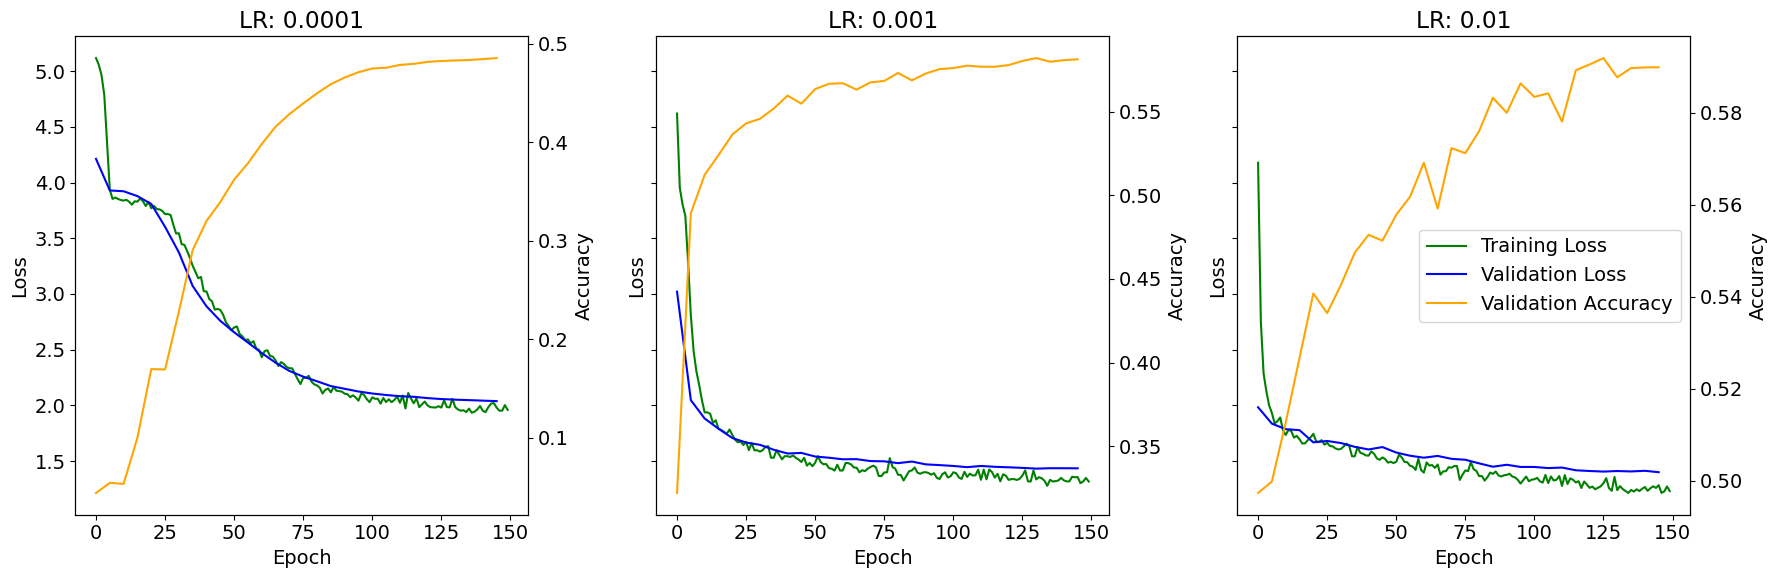
\includegraphics[width=1.0\textwidth]{figures/lr_search_cosine.png}
    \caption{Training graphs for the \emph{CRNN} with different learning rates and the \texttt{cosine} scheduler. The learning rate of $0.001$ seems to be the best, as it converges in a reasonable time and the validation accuracy increases in a stable fashion. While it may seem that running for more epochs may increase performance, this was not found to be the case empirically. The best model was often achieved around epoch 100.}\label{fig:lr_search_cosine}
\end{figure*}

\begin{table*}[h]
    \centering
    \begin{tabular}{lcccccc}
        \toprule
        lr & scheduler & acc & root & third & seventh & mirex \\
        \midrule
        0.01 & Cosine &  53.6 & 69.5 & 66.9 & 55.7 & 78.6 \\
        0.001 & Cosine & \emph{59.7} & \emph{78.3} & \emph{75.0} & \emph{62.0} & \emph{\textbf{79.8}} \\
        0.0001 & Cosine & 53.2 & 72.1 & 66.9 & 55.2 & 72.0 \\
        \midrule
        0.001 & Plateau & \textbf{59.9} & 78.4 & 75.2 & \textbf{62.2} & 79.7 \\
        0.001 & None & 59.8 & \textbf{78.7} &\textbf{75.5} & 62.0 & 78.8 \\
        \bottomrule
    \end{tabular}
    \caption{\emph{CRNN} model results with different learning rates and schedulers. Best results over learning rates are \emph{italicised} and best results over schedulers are in \textbf{boldface}. A learning rate of $0.001$ performs the best on all metrics. The differences between learning rate schedulers are so small that the choice between them is arbitrary. }\label{tab:crnn_lr}
\end{table*}


\subsection{Ablation on CRNN Model/Training}\label{app:crnn_ablation}

Using the best learning rate and learning rate scheduler from~\ref{app:learning_rate_scheduler}, we perform a random search over the number of layers in the GRU, the hidden size of the layers in the GRU the training patch segment length, the number of convolutional layers before the GRU, the kernel size of these layers and the number of channels outputted by each of these layers. The search is performed by independently and uniformly randomly sampling 50 points over discrete sets of possible hyperparameter values. 

Table~\ref{tab:crnn_hparams} shows a sample of the results. Results across hyperparameters are relatively stable. In general, increasing model complexity hurts performance and the differences between models are relatively small. Such small differences indicate that the model is learning something simple where increased model complexity does not help. It also seems that the choice of hyperparameters is somewhat arbitrary. The models do not utilise information from a larger context. Deeper layers with more parameters do not help performance. In fact, the parameters suggested by~\cite{StructuredTraining} perform just as well as the best-performing hyperparameter selection found in this random search. We therefore proceed with the same hyperparameters suggested by~\cite{StructuredTraining} as default for the remainder of experiments.

\begin{table*}[h]
    \centering
    \begin{tabular}{ccccccccccc}
        \toprule
        $L$ & $h$ & $k$ & $c$ & $g$ & $ch$ & acc & root & third & seventh & mirex \\
        \midrule
        23 & 231 & 5 & 1 & 1 & 1 & \textbf{59.8} & 78.2 & 74.7 & \textbf{62.0} & \textbf{79.9} \\
        11 & 150 & 7 & 2 & 1 & 3 & 59.6 & 78.5 & 75.0 & 61.9 & 79.2 \\
        43 & 222 & 11 & 2 & 2 & 2 & 59.5 & \textbf{78.7} & \textbf{75.2} & 61.8 & 78.9 \\
        \ldots & \ldots & \ldots & \ldots & \ldots & \ldots & \ldots & \ldots & \ldots & \ldots & \ldots \\
        34 & 159 & 14 & 4 & 2 & 1 & 56.9 & 75.5 & 72.2 & 59.1 & 77.7 \\
        \bottomrule
    \end{tabular}
    \caption{A subset of \emph{CRNN} model results on the large vocabulary with different hyperparameters. The best results for each metric are in boldface. $L$ is the length of training patches of audio in seconds, $h$ and $g$ are the hidden size and number of layers in the GRU respectively and $k$, $c$ and $ch$ are the kernel sizes, number of layers and number of channels in the CNN respectively. Models are ordered by their `Rank', calculated by adding the model's rank order over each metric and ordering by this total. Results across most hyperparameters are very similar. Comparing with the best results from the learning rate search in Table~\ref{tab:crnn_lr}, it seems that the parameters suggested by \cite{StructuredTraining} are good choices. Models with more parameters and longer input tend to perform worse, perhaps due to overfitting. This suggests that the model is learning something simple.}\label{tab:crnn_hparams}
\end{table*}

\subsection{Hop Lengths}\label{app:hop_lengths}

Different hop lengths have been used to calculate the CQT ranging from 512~\cite{ACRLargeVocab1} up to 4096~\cite{StructuredTraining}. In previous experiments we have used a hop length of $4096$ as is used by the authors of \emph{CRNN}~\cite{StructuredTraining}. Shorter frames would reduce the number of transition frames but require more computational cost. If frame lengths are too short, the Fourier transform may not be able to capture the harmonic structure of the audio.

In Table~\ref{tab:hop_lengths}, we test the effect of different hop lengths on the model's performance. We use a CQT with $216$ bins and a hop length of $512$, $1024$, $2048$, $4096$, $8192$ and $16384$. Results indicate that performance is similar for hop lengths of $4096$ and below. Performance suffers for greater hop lengths. While it could be argued that $2048$ does better than $4096$, this difference is small enough that it is not worth the increased computational cost. Models trained with a hop size of $2048$ take at least twice as long to train and evaluate as those trained on a hop size of $4096$.

\begin{table*}[h]
    \centering
    \begin{tabular}{lccccc}
        \toprule
        hop length & acc & root & third & seventh & mirex \\  
        \midrule
        512 & 60.1 & 78.3 & \textbf{75.5} & 62.4 & \textbf{80.0} \\
        1024 & 60.2 & \textbf{78.7} & 75.2 & 62.5 & 79.6 \\
        2048 & \textbf{60.3} & 78.5 & 75.2 & \textbf{62.6} & 79.6 \\
        4096 & 60.0 & 78.1 & 75.0 & 62.2 & 79.2 \\
        8192 & 57.9 & 76.2 & 72.9 & 60.1 & 79.3 \\
        16384 & 53.3 & 71.7 & 68.0 & 55.4 & 77.9 \\
        \bottomrule
    \end{tabular}
    \caption{Results over different hop lengths for CQT calculation. Any hop length in the range $512$ to $4096$ has similar performance. For frames that are any longer, performance suffers. This is likely caused by the requirement for the model to assign a single chord class to each frame. The longer the frame, the greater potential there is for multiple chords to be playing during the frame. }\label{tab:hop_lengths}
\end{table*}

\subsection{Output Smoothing}\label{app:output_smoothing}

The \emph{CRNN} with no smoothing predicts an average of $168$ transitions per song as opposed to the $104$ seen in the ground truth data. We implement a decoding step over the frame-wise probability vectors to smooth predicted labels. Common choices for decoding models include a conditional random field (CRF)~\cite{ACRLargeVocab1, BTC} and a hidden Markov model (HMM)~\cite{BalanceRandomForestACR}. 

We first implement a HMM. The HMM treats the frame-wise probabilities as emission probabilities and the chord labels as hidden states. \cite{CQTvsChroma} note that using a transition matrix with homogeneous off-diagonal entries in the transition matrix performs similarly to using a learned transition matrix. We adopt such a transition matrix for this HMM, with a parameter $\beta$ denoting the probability of self-transition and all other transition probabilities equal to $\frac{1-\beta}{C-1}$. Decoding then follows the Viterbi algorithm~\cite{Viterbi} over the summed forward and backward pass.

A plot of the effect of $\beta$ on the model's performance and the number of transitions per song is shown in Figure~\ref{fig:hmm_beta_search}. From this plot, we conclude that smoothing has little effect on the performance of the model while successfully reducing the number of transitions per song to that of the true labels. We select $\beta = 0.15$ for the remainder of experiments as it results in $102$ transitions per song while maintaining high performance. 

\begin{figure*}[ht]
    \centering
    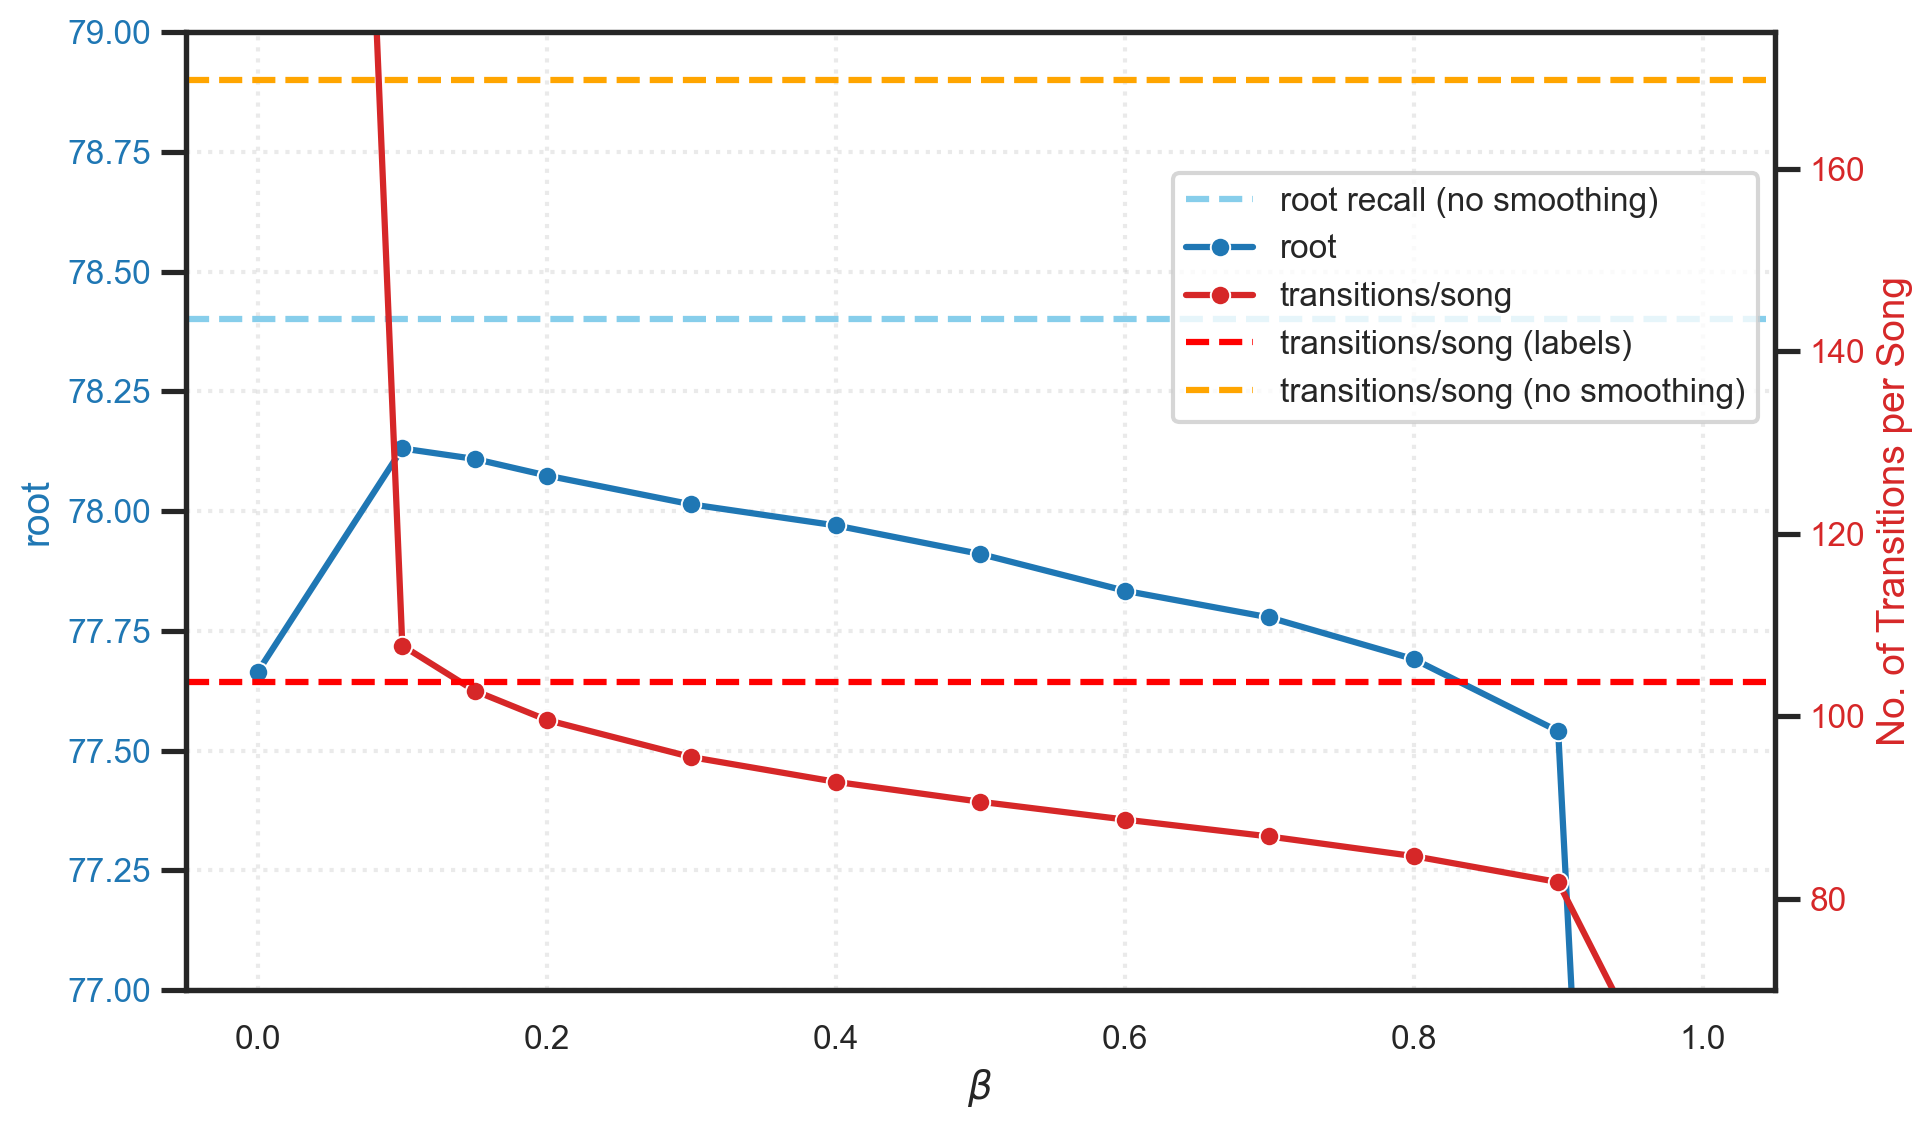
\includegraphics[width=0.8\textwidth]{figures/hmm_beta_vs_root_transitions.png}
    \caption{Effect of the HMM smoothing parameter $\beta$ on the \emph{CRNN} model. As we increase $\beta$, the number of transitions per song decreases. We choose $\beta = 0.15$ as it results in $102$ transitions per song, very close to the $104$ of the ground truth. Performance is stable across $\beta$ with a slight degradation for $\beta > 0.3$. Other performance metrics showed similarly stable results. }\label{fig:hmm_beta_search}
\end{figure*}

We also implement a linear chain CRF using \texttt{pytorch-crf}.\footnote{\url{https://github.com/kmkurn/pytorch-crf}} In contrast to the HMM, the CRF uses a learned transition matrix. Results comparing the HMM, CRF and no smoothing can be found in Table~\ref{tab:smoothers}. Both the CRF and HMM reduce the number of transitions per song to a similar level. The HMM outperforms the CRF with $3.5\%$ greater accuracy. The HMM has almost identical performance to the model with no smoothing. We hypothesise that the learned transition matrix allows the model to overfit to the chord sequences in the training set. Regardless of the explanation, we proceed with HMM smoothing.

\begin{table*}[h]
    \centering
    \begin{tabular}{lcccccc}
        \toprule
        smoother & acc & root & third & seventh & mirex & transitions/song\\  
        \midrule
        none & \textbf{60.0} & \textbf{78.1} & \textbf{75.0} & \textbf{62.3} & \textbf{79.2} & 167 \\
        HMM & \textbf{60.0} &\textbf{78.1} & \textbf{75.0} & \textbf{62.3} & \textbf{79.2} & \textbf{102} \\
        CRF & 56.5 & 75.5 & 72.5 & 58.6 & 76.2 & 100 \\
        \bottomrule
    \end{tabular}
    \caption{Results for the HMM and CRF smoothing methods with the \emph{CRNN}. The HMM has almost identical performance to the model with no smoothing. Smoothing must correct predictions for roughly the same amount of time as it introduces errors. However, it drastically reduces the number of transitions per song to an acceptable level. The CRF performs notably worse than the HMM. }\label{tab:smoothers}
\end{table*}

\subsection{Pitch Augmentation}~\label{app:pitch_augmentation}

Pitch augmentation can be done directly on the CQT~\cite{ACRLargeVocab1} or on the audio~\cite{BTC,StructuredTraining}. Although similar, these are not identical transformations as shifting the CQT takes place after discarding phase information and leaves empty bins behind, whereas audio pitch shifting can introduce other artefacts intended to preserve harmonic structure and maintain phase information.

When a sample is drawn from the training set, it is shifted with probability $p$. The shift is measured in semitones in the set $\{-5,-4\ldots -1, 1, \ldots 6\}$ with equal probability of each shift. This results in 12 times as much training data. Convergence is still reached in 150 epochs. Shifting the CQT matrix is done by moving all items up or down by the number of bins corresponding to the number of semitones in the shift. 

The remaining bins are filled with a value of -80dB. Audio shifting is done with \texttt{pyrubberband}.\footnote{\url{https://github.com/bmcfee/pyrubberband}}. CQTs are then calculated on the shifted audio. A plot of the effect of the shift probability $p$ on the model's performance can be found in Figure~\ref{fig:pitch_augmentation}.

Results show a clear trend that increasing $p$ improves performance. Shifting the audio provides a very similar effect to simply shifting the CQT. Choosing $p=0.9$ results in a $2.1\%$ increase in accuracy. The \texttt{mirex} score breaks the trend with performance varying over different values for $p$. The acc\textsubscript{class} metric also improves by more than $2\%$. This can be explained by the model becoming becoming root-invariant. With $p=0.9$, all potential roots become close to equally likely. We proceed with pitching shifting with $p=0.9$ on the CQT for the remainder of the experiments as it is computationally cheaper than shifting the audio.

Note that the weights for the weighted loss are calculated based on \emph{expected} counts, taking into account the shift probability $p$. We also test shifting on both the CQT and audio but the results are not different than shifting with either method alone. Unfortunately, it was not computationally feasible to test pitch shifting with generative features as the feature extraction over $12 * 1210 = 14,520$ songs is too expensive.

\begin{figure*}[h]
    \centering
    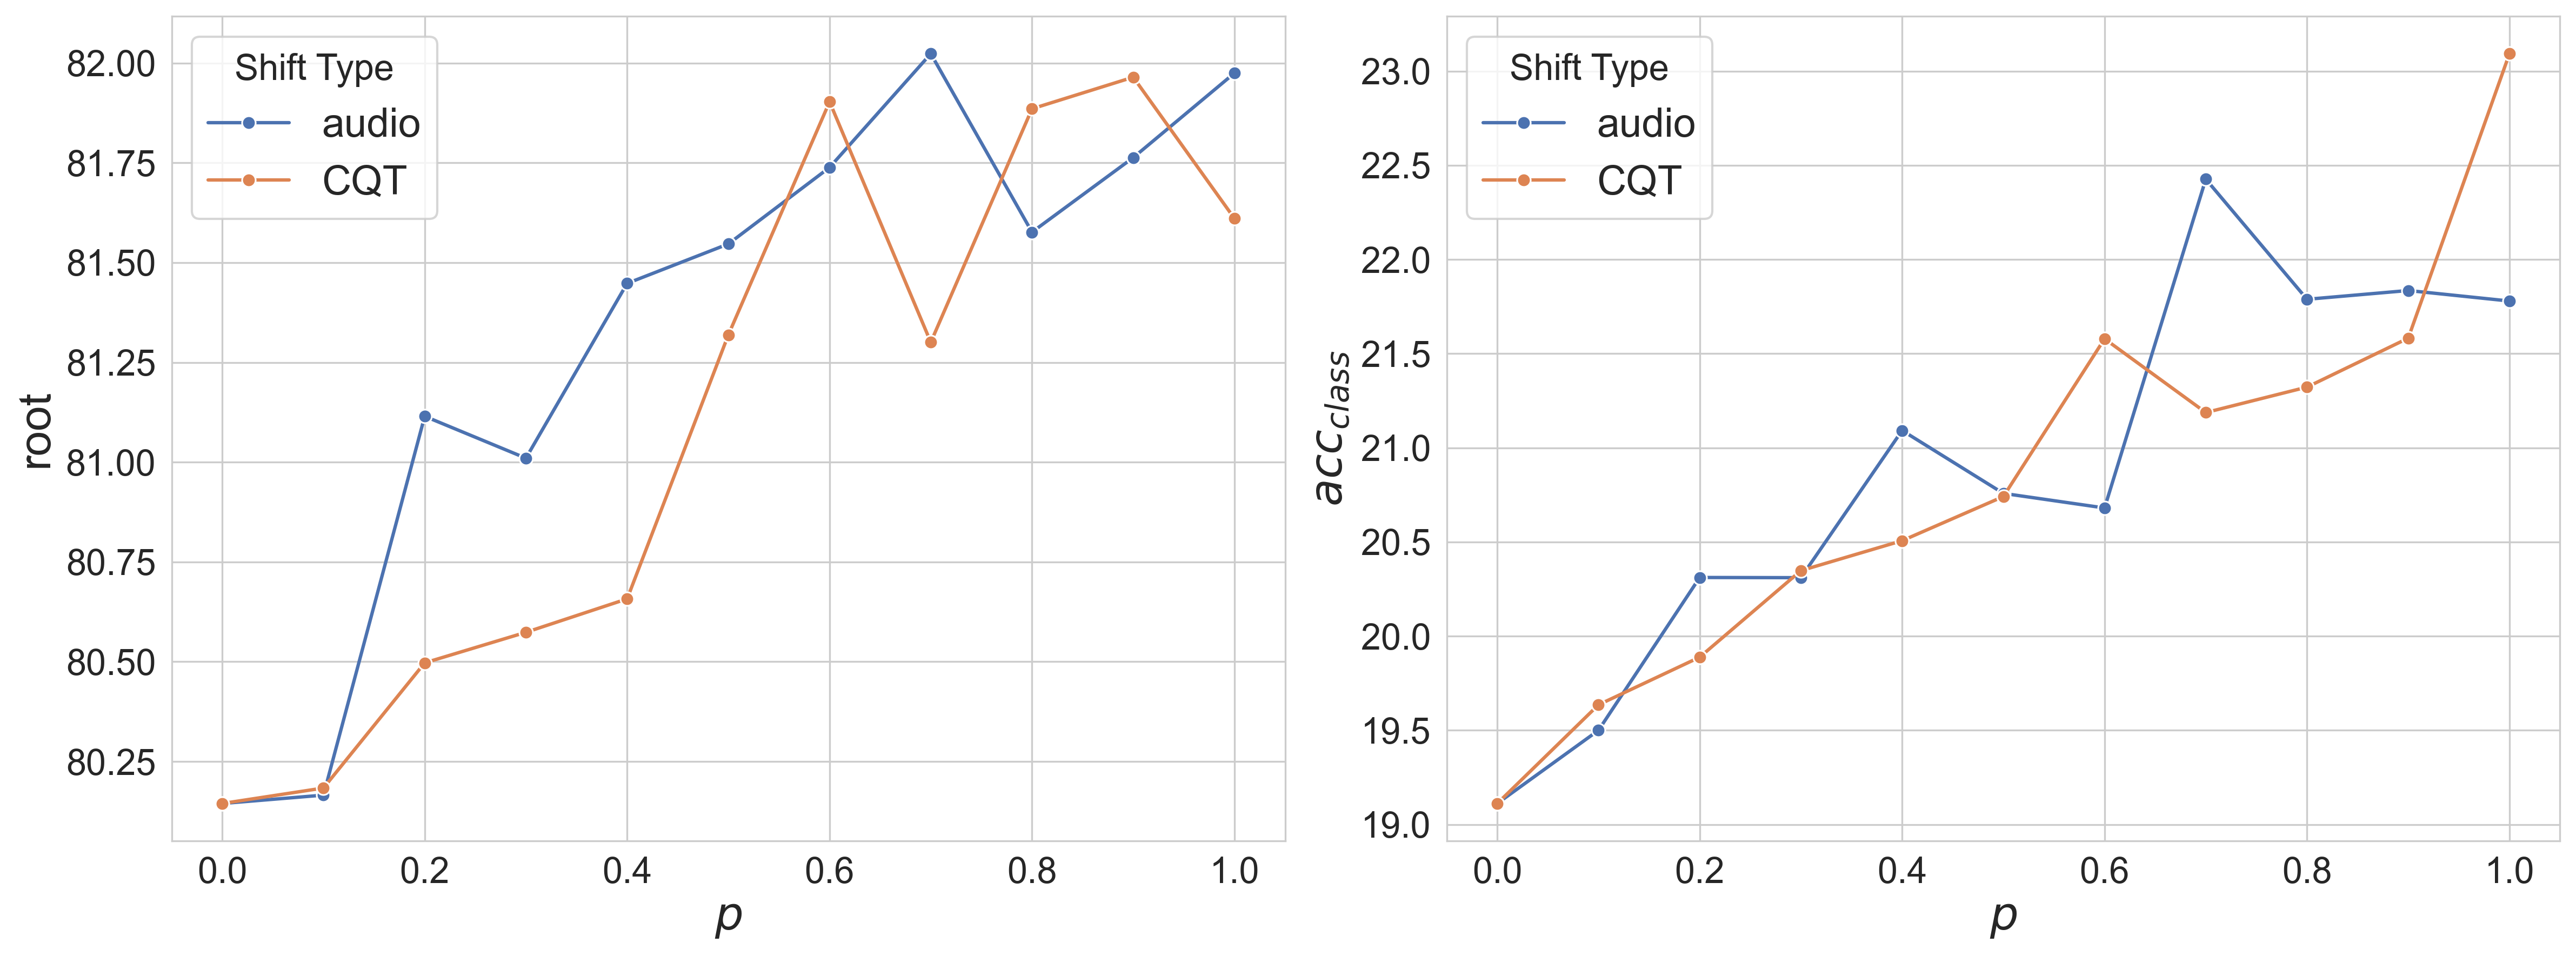
\includegraphics[width=1.0\textwidth]{figures/pitch_shift_analysis.png}
    \caption{Effect of pitch shift probability $p$ on \texttt{root} (left) and acc\textsubscript{class} (right). Pitch shifting provides a clear increase in performance. Shifting the audio or the CQT has a similar effect. We choose $p=0.9$, which is close to making the model root-invariant.}\label{fig:pitch_augmentation}
\end{figure*}


\subsection{Weighted Loss}\label{app:weighted_loss}

One of the greatest difficulties in ACR is the few instances of rare chord qualities. Two standard methods for dealing with long-tailed distributions are weighting the loss function and over-sampling. \cite{CurriculumLearning} also explore the use of curriculum learning as a form of re-sampling which we do not explore here because they report only minor performance gains. Sampling is explored by~\cite{BalanceRandomForestACR}, but they use a different model based on pre-computing chroma vectors and re-sampling these chroma vectors for use in training a random forest for frame-wise decoding. In our setting, re-sampling training patches of audio may be interesting to explore but is left as future work. It would require a complex sampling scheme as frames cannot be sampled independently. 

Weighting has been explored by~\cite{ACRLargeVocab1}. We employ a similar but simpler implementation here. A standard method of weighting is to multiply the loss function by the inverse frequency of the class of the current training sample, with a parameter controlling the strength of the weighting. This is defined in Equation~\ref{eq:weighting}.

\begin{equation}\label{eq:weighting}
    w_c = \frac{1}{{(\text{count}(c) + 10)}^\alpha}
\end{equation}

where $w_c$ is the weight for chord $c$, $\text{count}(i)$ is the number of frames with chord $c$ in the dataset and $\alpha$ is a hyperparameter controlling the strength of weighting. $\alpha=0$ results in no weighting and increasing $alpha$ increases the severity of weighting. We add $10$ in the denominator to avoid dividing by $0$ and to diminish the dominating effect of chords with very few occurrences. We then define normalised weights $w_c^*$ in Equation~\ref{eq:weighted_loss}.


\begin{equation}\label{eq:weighted_loss}
    w_c^* = \frac{w_c}{s} \text{ where } s = \frac{\sum_{c\in \mathcal{C}} \text{count}(c)\cdot w_c}{\sum_{c\in \mathcal{C}} \text{count}(c)}
\end{equation}

Where $\mathcal{C}$ is the set of all chords in the vocabulary. This keeps the expected weight over samples at $1$ such that the effective learning rate remains the same. These values are calculated over the training set. We test values of $\alpha$ in the set \{0, 0.05, 0.1, \ldots, 0.95, 1\}. The plot in Figure~\ref{fig:weighted_loss} illustrates the effect of the weighting on the model's performance. We find that increasing $\alpha$ improves \texttt{acc}\textsubscript{class} but decreases \texttt{root} accuracy. Choosing $\alpha = 0.3$ maximises \texttt{acc}\textsubscript{class} without hurting root accuracy which we carry forward to subsequent experiments.

\begin{figure*}[h]
    \centering
    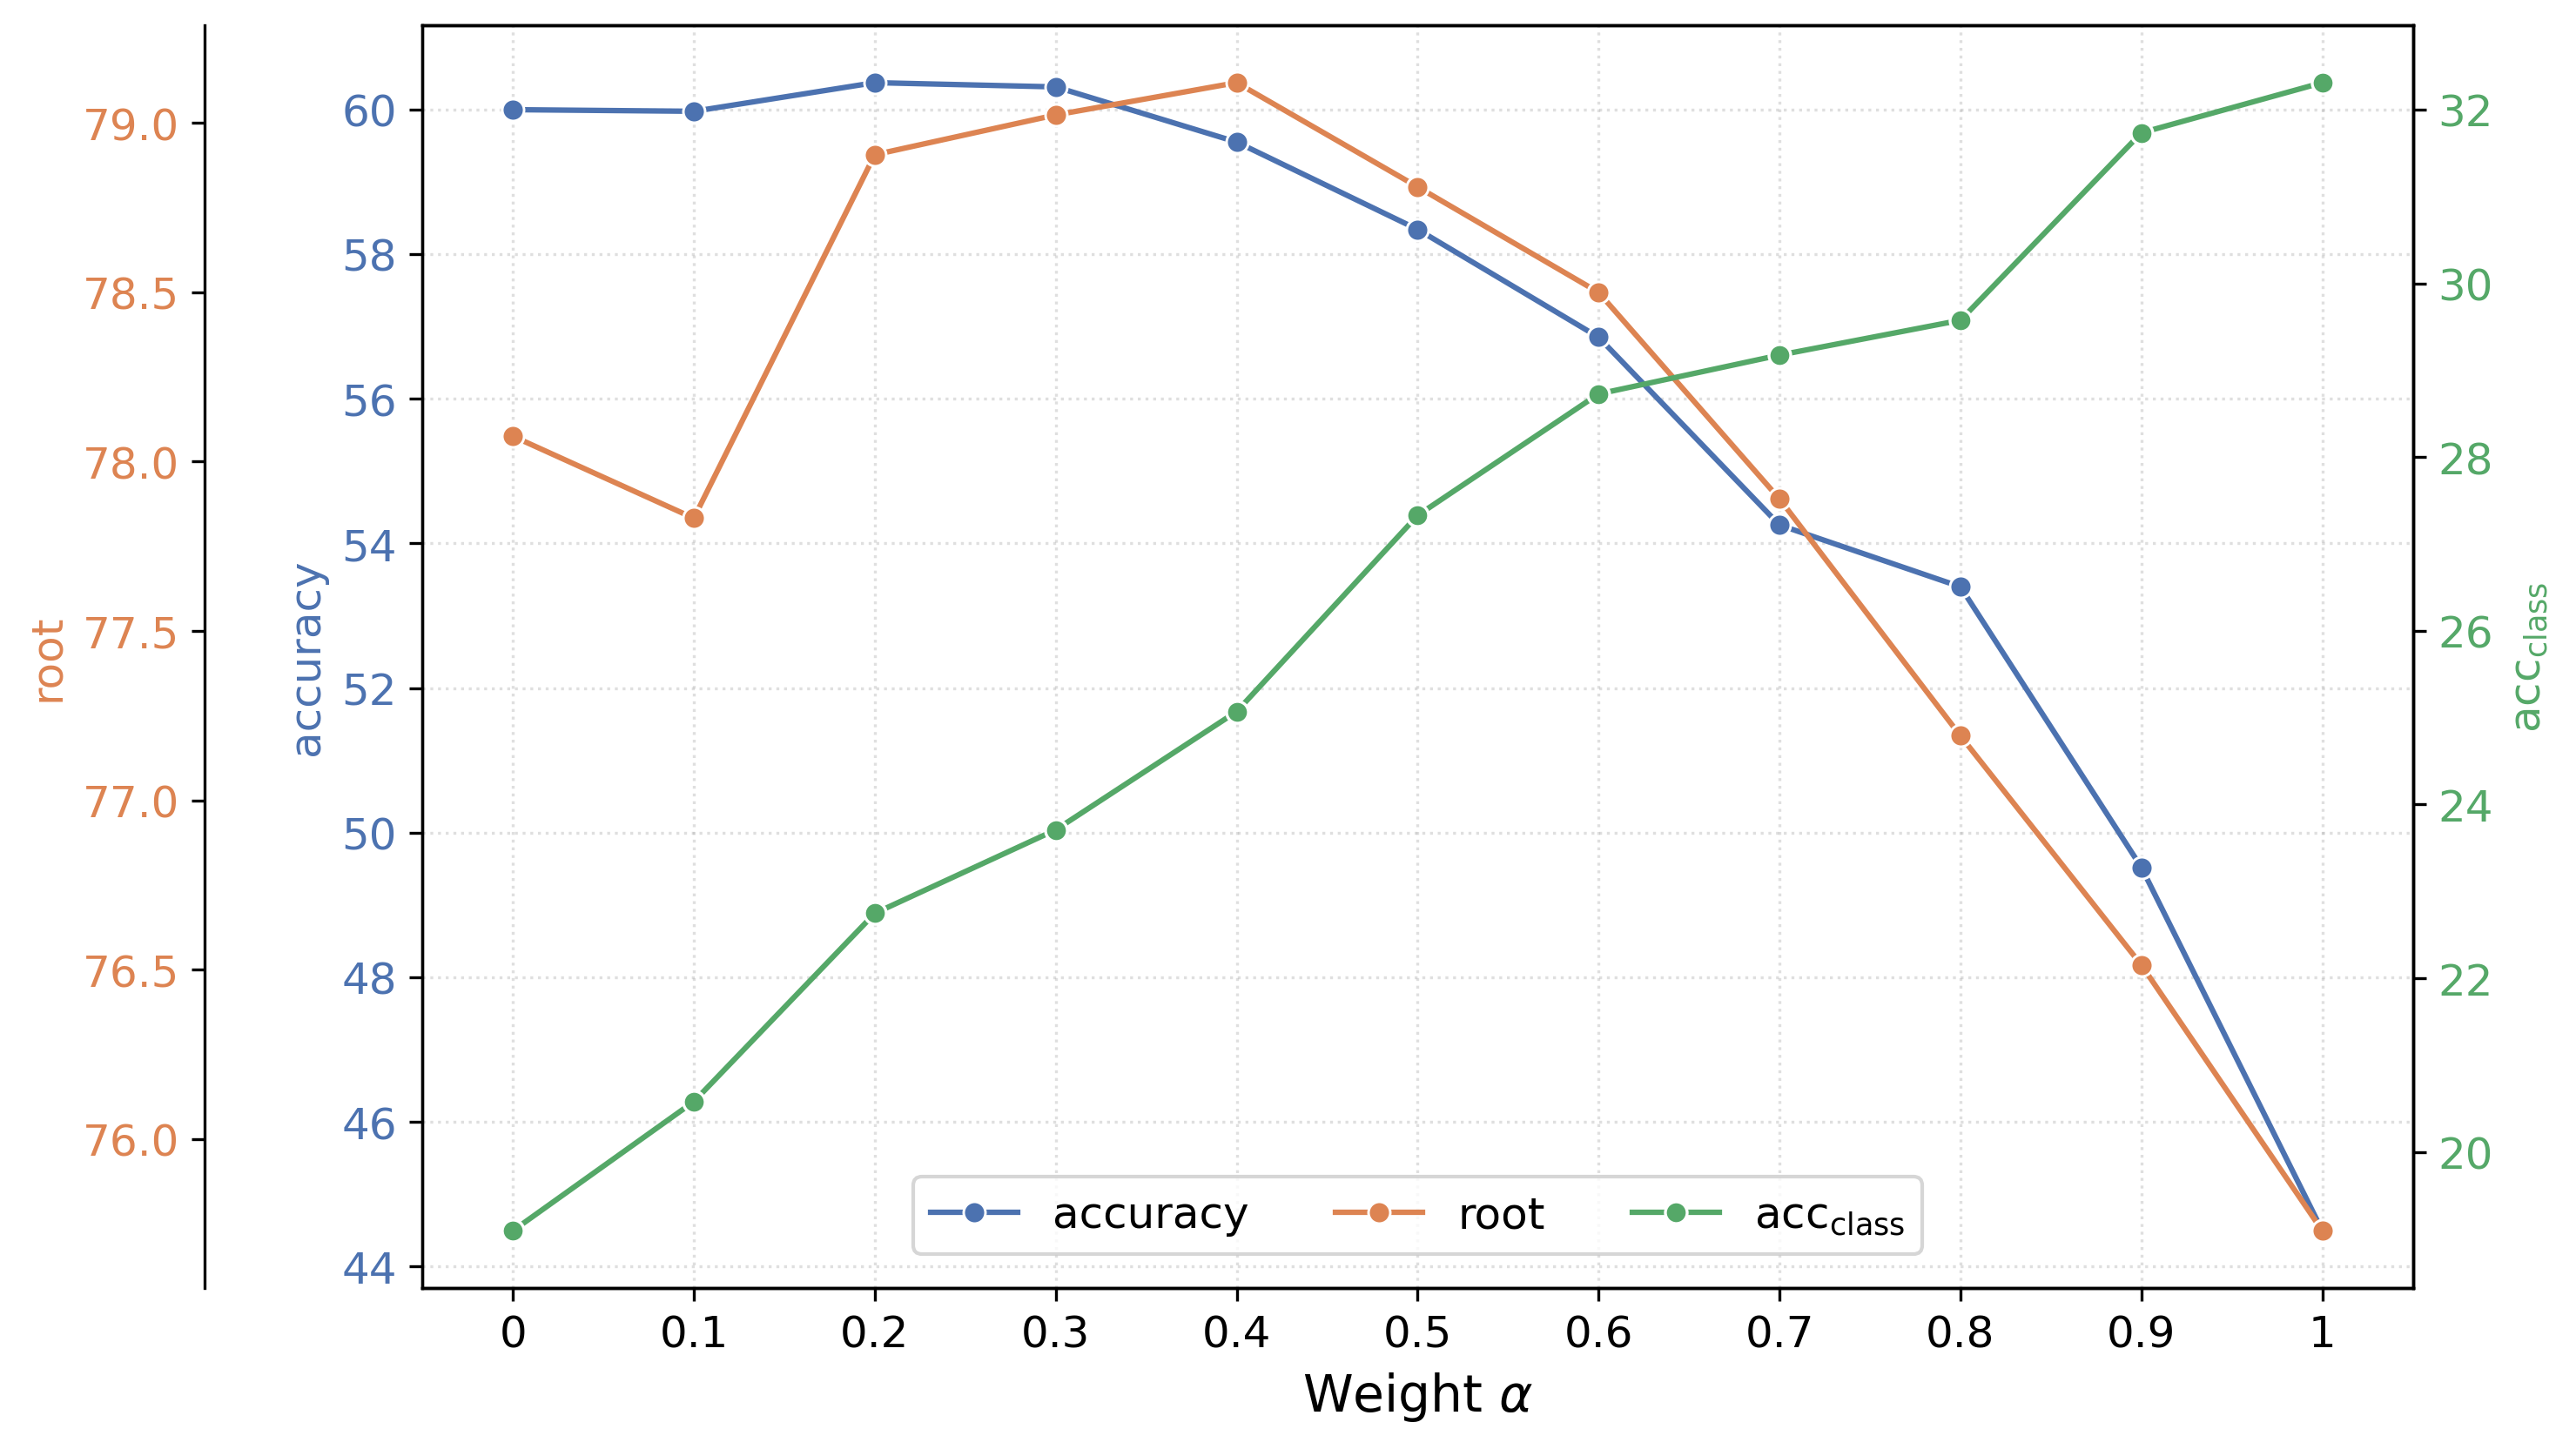
\includegraphics[width=0.8\textwidth]{figures/weight_alpha_search_trim.png}
    \caption{Effect of weighted loss on the \emph{CRNN} model with varying $\alpha$. As we increase $\alpha$, \texttt{acc}\textsubscript{class} improves accuracy and \texttt{root} decreases. We claim there is a sweet spot where very little overall performance is sacrificed for better class-wise accuracies. We select $\alpha = 0.3$. The \texttt{root} and \texttt{third} metrics improve and less than $3\%$ is lost on other metrics while mean class-wise accuracy improves by $6\%$.}\label{fig:weighted_loss}
\end{figure*}

Weighting the loss function also slightly increases the number of transitions predicted per song. This may be because occasional sharp gradient updates cause more extreme probability outputs. we increase the HMM smoothing parameter $\beta$ to $0.2$ to bring the number of transitions per song to $104$.

\subsection{Structured Loss}\label{app:structured_loss}

\cite{StructuredTraining} propose a structured loss function. They introduced additional targets for the root, bass and pitch classes. We follow a similar method but do not include the bass as the current chord vocabulary does not consider inversions. The idea behind this loss term is to explicitly task the model with identifying the components of a chord we care about. This can allow the model to exploit structure in the chord vocabulary such as shared roots and pitch classes, rather than all symbols being predicted independently.

The root can be any of the 12 notes in the Western chromatic scale, \texttt{N} or \texttt{X}, creating a 14-dimensional classification problem. The 12 pitch classes each represent a single binary classification problem. Two fully connected layers calculate a 14-dimensional vector and 12-dimensional vector from the hidden representation outputted from the GRU for the root and pitch classes, respectively. Finally, these representations are concatenated with the GRU representations and fed into the final fully connected layer to predict the chord symbol.

The mean cross-entropy loss is calculated in each case. These are summed to form the \emph{structured loss}. The final loss is a convex combination of the original loss and the structured loss as defined in Equation~\ref{eq:structured_loss}.

\begin{equation}\label{eq:structured_loss}
    L = \gamma L_{chord} + (1-\gamma)(L_{root} + L_{pitch})
\end{equation}

Where $L$ is the overall loss, $L_{chord}$ is the cross-entropy loss over chords symbols, $L_{root}$ is the cross-entropy loss targeting the root, $L_{pitch}$ is mean binary cross-entropy over each of the pitch classes. $\gamma$ is a hyperparameter controlling the weighting of the original loss. 

We test models with $\gamma\in\{0, 0.1 \ldots 0.9\}$. Choosing $\gamma=0.7$ improves accuracy by $1.3\%$ while \texttt{mirex} worsens by $0.3\%$. Accuracy with \texttt{third} increases by $1.7\%$ and on \texttt{seventh} by $1.3\%$. Generally, greater $\gamma$ improves accuracy metrics while \texttt{mirex} results are noisy. A plot of the trend can be found in Figure~\ref{fig:structured_loss}. We keep $\gamma=0.7$ from now on based on peak accuracy.

\begin{figure*}[h]
    \centering
    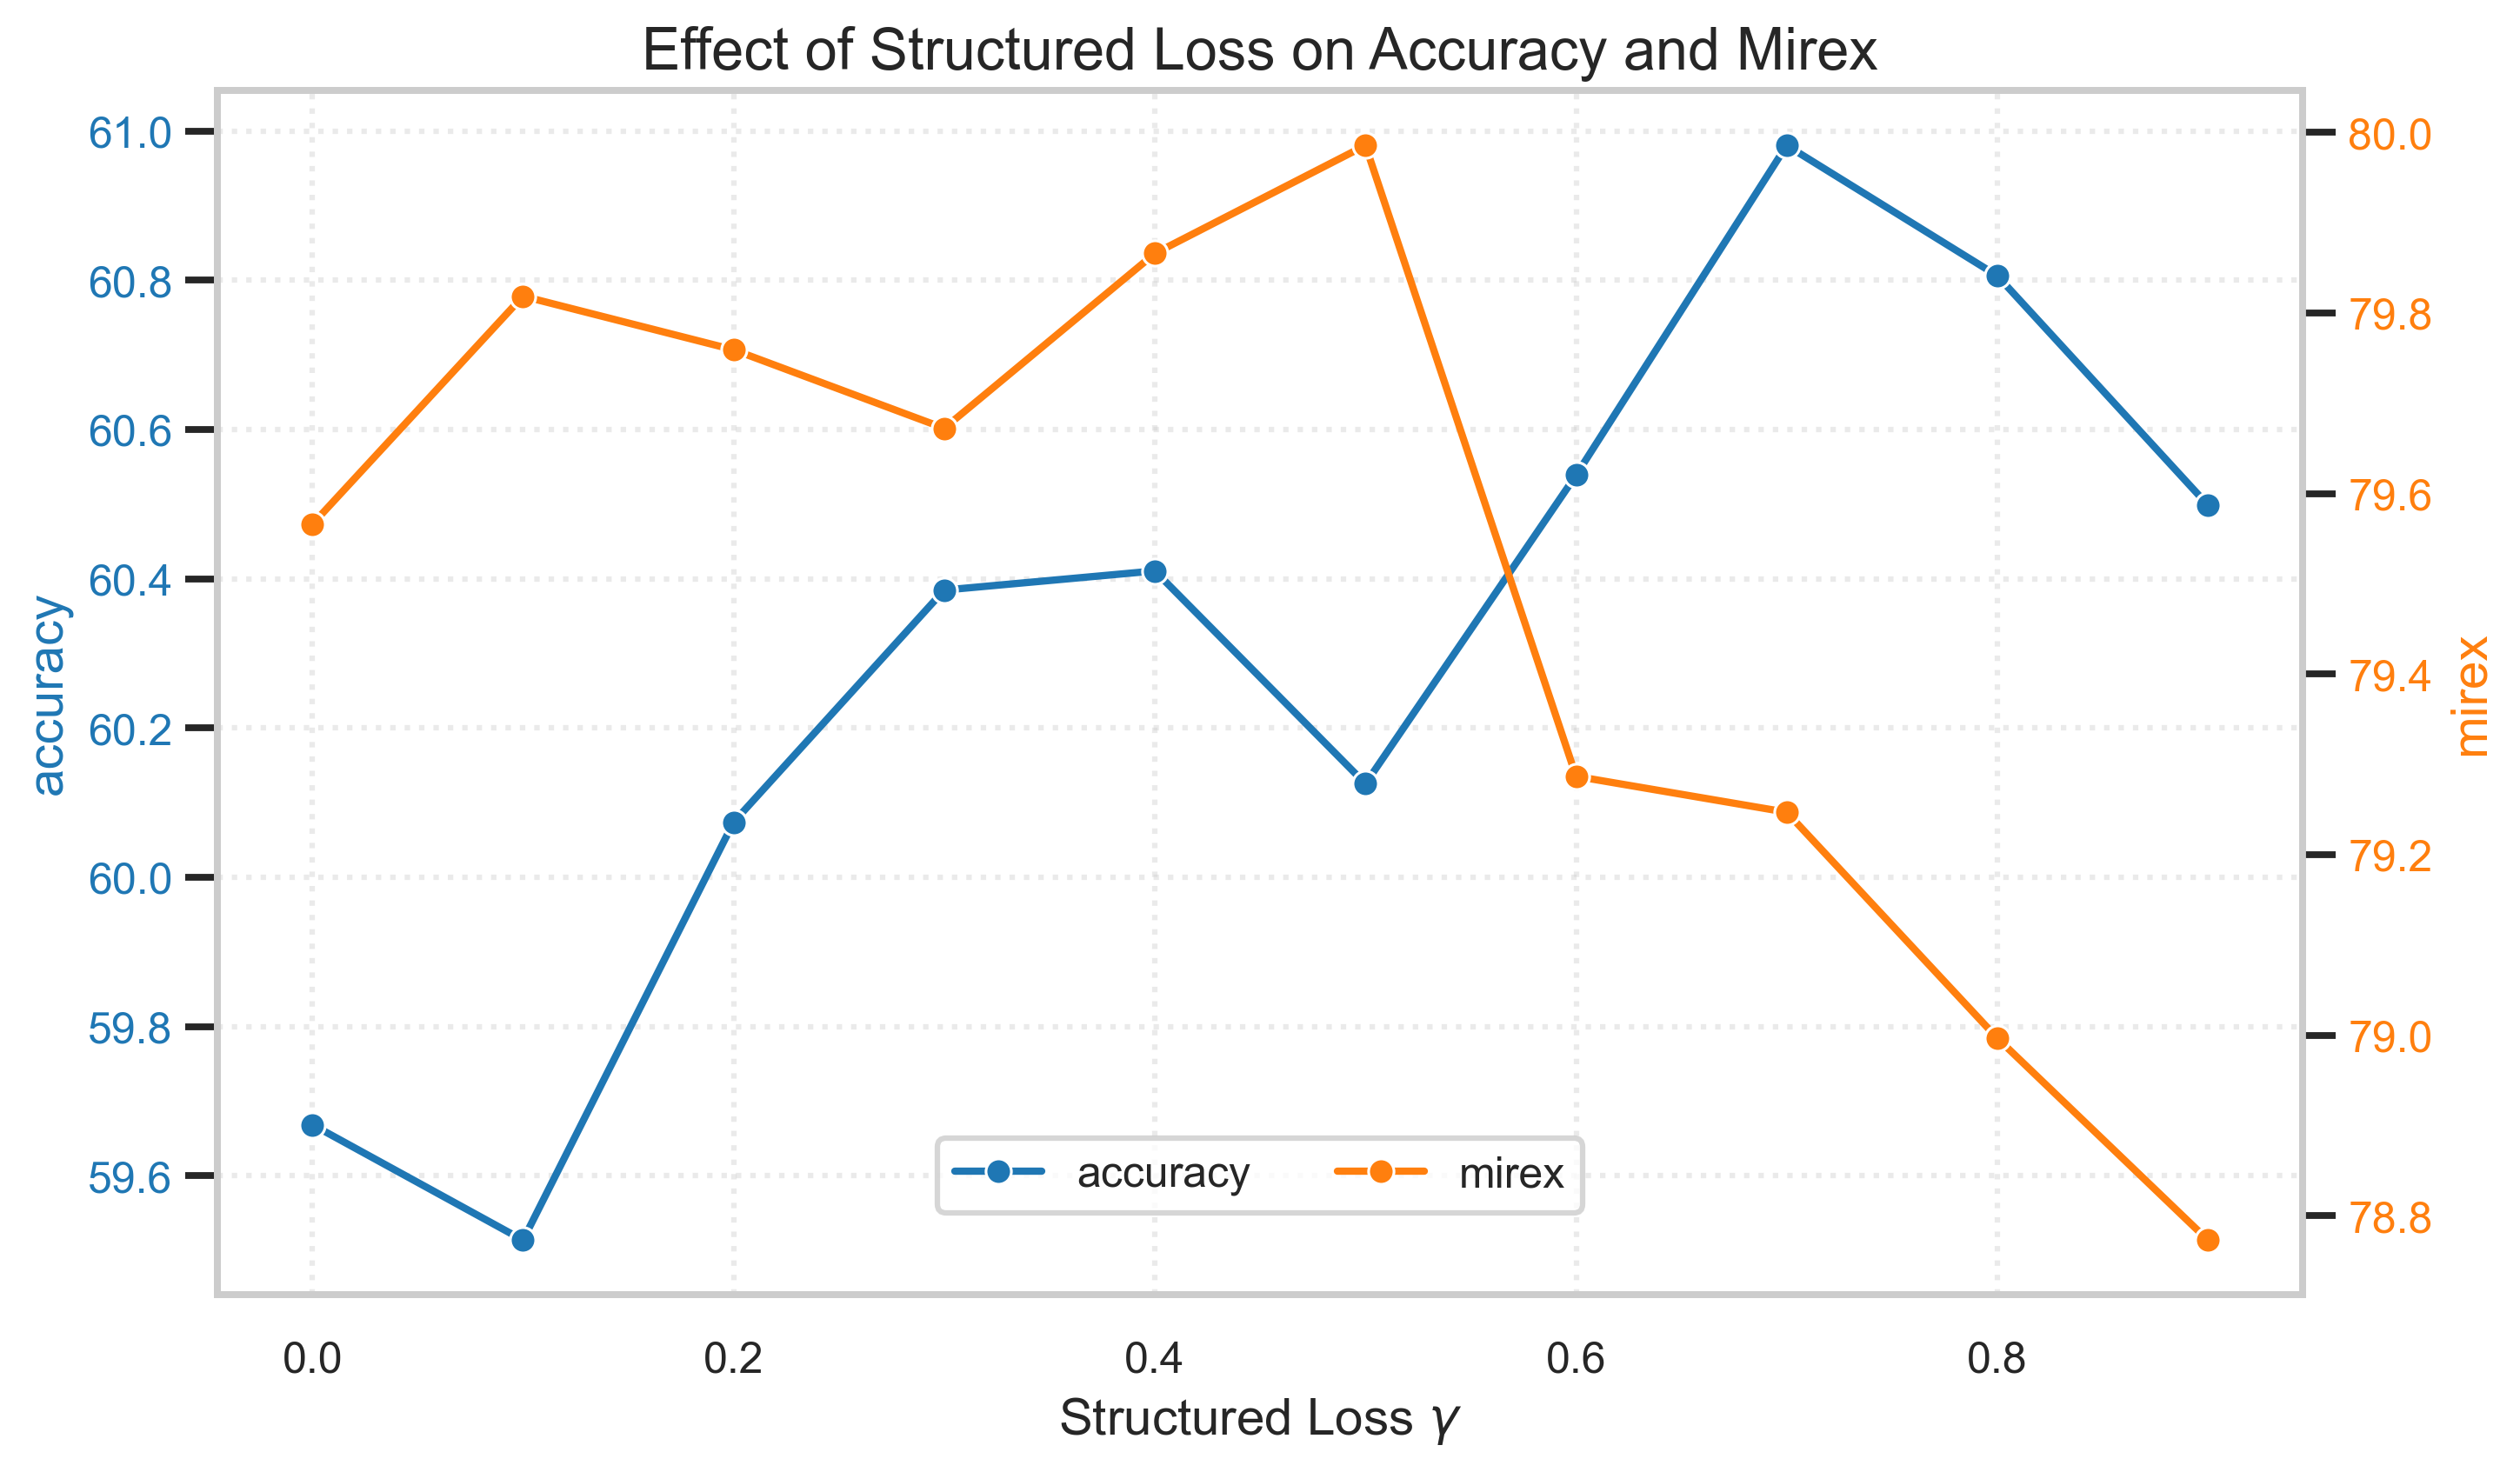
\includegraphics[width=0.8\textwidth]{figures/structured_loss_accuracy.png}
    \caption{Effect of structured loss on the \emph{CRNN} model with varying $\gamma$. As we increase $\gamma$, accuracy improves but \texttt{mirex} behaves erratically, worsening at the higher end. The other metrics behave similarly to accuracy. We choose $\gamma=0.7$ based on peak accuracy. }\label{fig:structured_loss}
\end{figure*}

\subsection{Details of Generative Feature Extraction}\label{app:generative_feature_extraction}

Overlapping $5$ second chunks of audio were fed through MusicGen in a batched fashion. This first requires passing the audio through the pre-trained Encodec audio tokeniser~\cite{Encodec}. These are then fed through the language model. We take the output logits as the representation for each frame. The model outputs logits in four `codebooks', each $2048$-dimensional vectors, intended to represent different granularities of detail in the audio. Audio segments are overlapped such that every frame has context from both directions. The multiple representations for each frame are averaged. Finally, these representations are upsampled. The model operates at a frame rate of 50Hz. To compute a representation with the same frame length as the CQT, we take the mean over the frames outputted by the model closest to the centre of the CQT frame. In case averaging over frames dampened the signal, we also tried linearly interpolating between the two closest frames outputted by the model. However, this was empirically found to perform slightly worse. Results can be found in Appendix~\ref{app:linear_interpolation_vs_area_averaging}. This feature extraction required the use of NVIDIA RTX A6000 GPUs. The extraction process took approximately 4 hours for each model over the entire dataset.

\subsection{Upsampling Methods in Generative Feature Extraction}\label{app:linear_interpolation_vs_area_averaging}

Table~\ref{tab:linear_interpolation_vs_area_averaging} compares linear interpolation and area averaging for upsampling generative features. The results are nearly identical across all metrics, though area averaging yields consistently small improvements. Based on this, we use area averaging to align model frames with CQT frames in subsequent experiments.

\begin{table*}[h]
    \centering
    \begin{tabular}{cccccc}
        \toprule
        upsample & accuracy & root & third & seventh & mirex  \\  
        \midrule
        area & \textbf{59.4} & \textbf{77.8} & \textbf{74.6} & \textbf{61.7} & \textbf{78.1} \\
        lerp & 58.4 & 77.7 & 74.0 & 60.6 & 78.2 \\
        \bottomrule
    \end{tabular}
    \caption{Comparison of generative feature extraction with linear interpolation and area averaging for the musicgen-large and a linear projection down to $64$ dimensions and averaging over the four codebooks. The results are very similar, but the area averaging method is slightly better in all metrics. We therefore choose to continue averaging over model frames in order to upsample to CQT frames.}\label{tab:linear_interpolation_vs_area_averaging}
\end{table*}

\subsection{Generative Feature Low-Dimensional Projection}\label{app:projection_dimensionality}

Table~\ref{tab:projection_dimensionality} shows that performance is largely insensitive to the projection dimension $d$, with only minor fluctuations across metrics. While $d=64$ achieves the best overall results, the differences are small and likely within optimisation variance, so no strong conclusion can be drawn about the optimal dimensionality.

\begin{table*}[h]
    \centering
    \begin{tabular}{cccccc}
        \toprule
        $d$ & accuracy & root & third & seventh & mirex  \\  
        \midrule
        16   & 58.4       & 77.6       & \textbf{74.5} & 60.6       & 77.2       \\
        32   & 57.8       & 77.5       & 73.6          & 60.0       & 77.8       \\
        64   & \textbf{59.2} & 77.5    & 74.3          & \textbf{61.4} & \textbf{77.9} \\
        128  & 58.1       & 77.0       & 73.6          & 60.3       & 77.4       \\
        256  & 58.7       & 77.6       & 74.3          & 60.9       & 77.5       \\
        512  & 58.3       & \textbf{77.9} & 74.3      & 60.6       & 77.6       \\
        1024 & 58.4       & 76.7       & 73.5          & 60.7       & 76.7       \\ 
        \bottomrule
    \end{tabular}
    \caption{Generative feature extraction with different projection dimensions, $d$. All results use the musicgen-large model and average across the four codebooks. There are no large differences between the different dimension reductions. We take $d=64$ as it performs the best, but there is no evidence that this is not due to randomness in the optimisation process. }\label{tab:projection_dimensionality}
\end{table*}

\subsection{Generative Features with Different Models}\label{app:generative_feature_extraction_models}

Table~\ref{tab:musicgen_pivot} compares generative features from different models and finds minimal variation in accuracy. The small model performs comparably to the large one, suggesting similar useful information in their representations. Notably, the chord-conditioned model does not outperform the melody model, indicating that chord conditioning provides limited benefit in this setting.

\begin{table*}[h]
    \centering
    \begin{tabular}{lc}
        \toprule
        model  & acc  \\
        \midrule
        large  & \textbf{60.2} \\
        small  & 59.8 \\
        melody & 59.9 \\
        chord  & 59.7 \\
        \bottomrule
    \end{tabular}
    \caption{Results for generative features extracted from MusicGen~\cite{MusicGen} and MusiConGen~\cite{MusiConGen} models with different musicgen-models. Only accuracy is reported as the other metrics are qually similar. These models are musicgen-large, musicgen-small, musicgen-melody and MusiConGen, referred to as large, small, melody and chord respectively. There are very few differences between the models. This suggests that the small model has just as much information in its internal representations that is useful for identifying chords as the other models. Another point of note is the comparison between chord and melody. The chord model is a chord-conditioned fine-tuned version of melody. It is surprising that the chord-conditioning did not help compared to the non chord-conditioned model.}\label{tab:musicgen_pivot}
\end{table*}

\subsection{Generative Features with Different Codebook Reductions}\label{app:generative_feature_extraction_reductions}

Table~\ref{tab:reduction_accuracy} evaluates different codebook reduction strategies and shows broadly similar performance across methods. Averaging yields the highest accuracy, while individual codebooks such as \texttt{codebook\_0} and \texttt{codebook\_3} perform slightly worse, motivating the choice of averaging in subsequent experiments.

\begin{table*}[h]
    \centering
    \begin{tabular}{lc}
        \toprule
        reduction   & accuracy \\  
        \midrule
        concat       & 58.9     \\
        codebook\_2  & 58.9     \\
        codebook\_3  & 57.5     \\
        codebook\_1  & 59.0     \\
        codebook\_0  & 58.1     \\
        avg          & \textbf{59.4}     \\
        \bottomrule
    \end{tabular}
    \caption{Accuracy for different codebook reduction methods. Other metrics are omitted as they do not provide more information. All results are for musicgen-large with reduction down to $64$ dimensions. Reductions of the form `codebook\_$n$' refer to training on codebook of index $n$ from the model. Performance is similar across reductions except for codebook\_0 and codebook\_3 which perform worse. We choose the averaging reduction based on maximum accuracy. }\label{tab:reduction_accuracy}
\end{table*}

\subsection{Spectrogram Variants}\label{app:spectrogram_variants}

It is standard practice in ACR to use a CQT as input. However, \cite{20YearsofACR} raise the question of whether the CQT is truly the best choice. They suggest that the pitch-folding of the CQT may distort the harmonic structure of notes. By contrast, \cite{MelodyTranscriptionViaGenerativePreTraining} use a mel-spectrogram in place of a CQT. 

We test four spectrogram variants in Table~\ref{tab:spectrograms}. These include the standard CQT, mel-spectrogram and linear spectrogram. We also calculate a chroma-CQT to test whether the model is using information from multiple octaves better than a hand-crafted algorithm. The chroma-CQT is calculated by summing CQT values across octaves. Spectrogram calculations are all implemented in \texttt{librosa}~\cite{librosa}. We use $216$ bins for the CQT and mel spectrograms and $2048$ fast Fourier transform (FFT) bins for the linear spectrogram with a hop length of $4096$ for all. 

Results show that CQTs are the best choice. This raises questions as to the validity of the conclusions drawn by \cite{MelodyTranscriptionViaGenerativePreTraining}. They claim that their generative features are better than hand-crafted features. However, they only compare to mel-spectrograms which may not perform as well as CQTs for the related task of melody recognition. The CQT is also better the chroma-CQT. We can be confident that the model is using information from multiple octaves more efficiently than the simply summing across octaves.

\begin{table*}[h]
    \centering
    \begin{tabular}{lccccc}
        \toprule
        spectrogram & acc & root & third & seventh & mirex \\  
        \midrule
        CQT & \textbf{60.2} & \textbf{78.4} & \textbf{75.3} & \textbf{62.5} & \textbf{79.5} \\
        chroma-CQT & 50.1 & 71.4 & 65.7 & 52.0 & 69.8 \\
        mel & 52.7 & 69.1 & 66.3 & 54.6 & 70.6 \\
        linear & 51.2 & 66.1 & 63.0 & 53.1 & 73.8 \\
        \bottomrule
    \end{tabular}
    \caption{Results for CQT, chroma-CQT, mel and linear spectrograms. The CQT is certainly the best feature. The other all perform similarly on accuracy and \texttt{mirex}, but the chroma-CQT does comparatively at identifying thirds and sevenths. }\label{tab:spectrograms}
\end{table*}


\subsection{Synthetic Data Generation}\label{app:synthetic_data_gen}

To generate a song, we sample a BPM from a normal distribution with mean $117$ and standard deviation $27$, clipped to lie in the range $[60,220]$. These values are calculated from the training set so as to stay roughly in-distribution. We then sample a song description from a set of $20$ generated by ChatGPT. The descriptions outline a genre, mood and instrumentation. Descriptions include only jazz, funk, pop and rock, which were all part of the fine-tuning training set for MusiConGen. The model does not output melodic vocals, owing to the lack of vocal music in the pre-training and fine-tuning data. Finally, we generate a jazz chord progression using the theory of functional harmony~\cite{GenerativeGrammarJazz}. The process generates a very different chord distribution than the one in \emph{pop} with many more instances of upper extensions and rare qualities. This is intended to provide the model with many more instances of rare chords.

\textbf{Chord Sequence Generation:} The theory of functional harmony is a set of rules that govern the relationships between chords in a piece of music. While these rules are not always followed, many chord progressions can be parsed and broken down into the rules that have been followed to create them. The rules are based on the relationships between the chords and the keys they are in. For example, a chord progression that moves from a tonic chord to a dominant chord is said to be following the rule of \emph{dominant function}. This is a common rule in jazz music and is often used to create tension and resolution in a piece of music.

We first decide whether we are in major or minor, each with probability $0.5$. We then uniformly sample a tonic from the set of notes in the Western chromatic scale. From this tonic, seven functional chords are decided before sequence generation. These are all probabilistic. For example, the tonic chord is always the tonic, but the dominant chord can be of \texttt{maj}, \texttt{7}, \texttt{sus4}, \texttt{aug} or \texttt{dim7} qualities. The probabilities are user-tuned but do not matter very much to the funcionality of the synthetic dataset. 

For chord sequence generation, various rules are followed in a probabilistic manner. Progressions have a random length, uniformly sampled in the range $[4, 10]$.

\begin{itemize}
    \item Tonic (I) may move to predominant chords (ii, IV, vi) or occasionally mediant (iii).
    \item Predominant chords (ii, IV) resolve to the dominant (V).
    \item Dominant (V) usually cadences back to tonic (I) or sometimes moves to vi.
    \item Tonic substitute (vi) leads to ii or iii.
    \item Mediants (iii) feed into vi.
    \item Unspecified or fallback transitions are routed toward ii to maintain forward motion.
\end{itemize}

A time-aligned chord sequence is then calculated in a similar format to that provided by the \texttt{jams} package. This assumes that each chord is played for one bar, that the BPM is always followed, and that MusiConGen simply loops over the chord progression if the end is reached. These assumptions were found to hold on manually inspected examples.

For further details and exact probabilities used, please refer to the provided code.\footnote{\url{https://github.com/PierreRL/LeadSheetTranscription/blob/main/src/data/synthetic_data/chord_sequence.py}}

\subsection{Calibration to Handle Distribution Shift}\label{app:calibration}

To correct for the distribution shift between synthetic training data and the \emph{pop} train split, we estimate the empirical class probabilities in each domain---\(P_{\text{train}}(y)\) and \(P_{\text{pop}}(y)\)---and rescale the model’s logits by the ratio
\begin{equation}
r(y)\;=\;\frac{P_{\text{pop}}(y)}{P_{\text{train}}(y)}.
\end{equation}

In order for calibration to be root invariant, we take the mean ratio over chords that share the same quality, and a single calibration factor \(r_q\) is applied to every chord with that quality. Note that the model's outputs are in logits so the log ratio is added in implementation. Figure~\ref{fig:calibration} shows the calibration of the model's outputs to account for distribution shift.

\begin{figure*}[h]
    \centering
    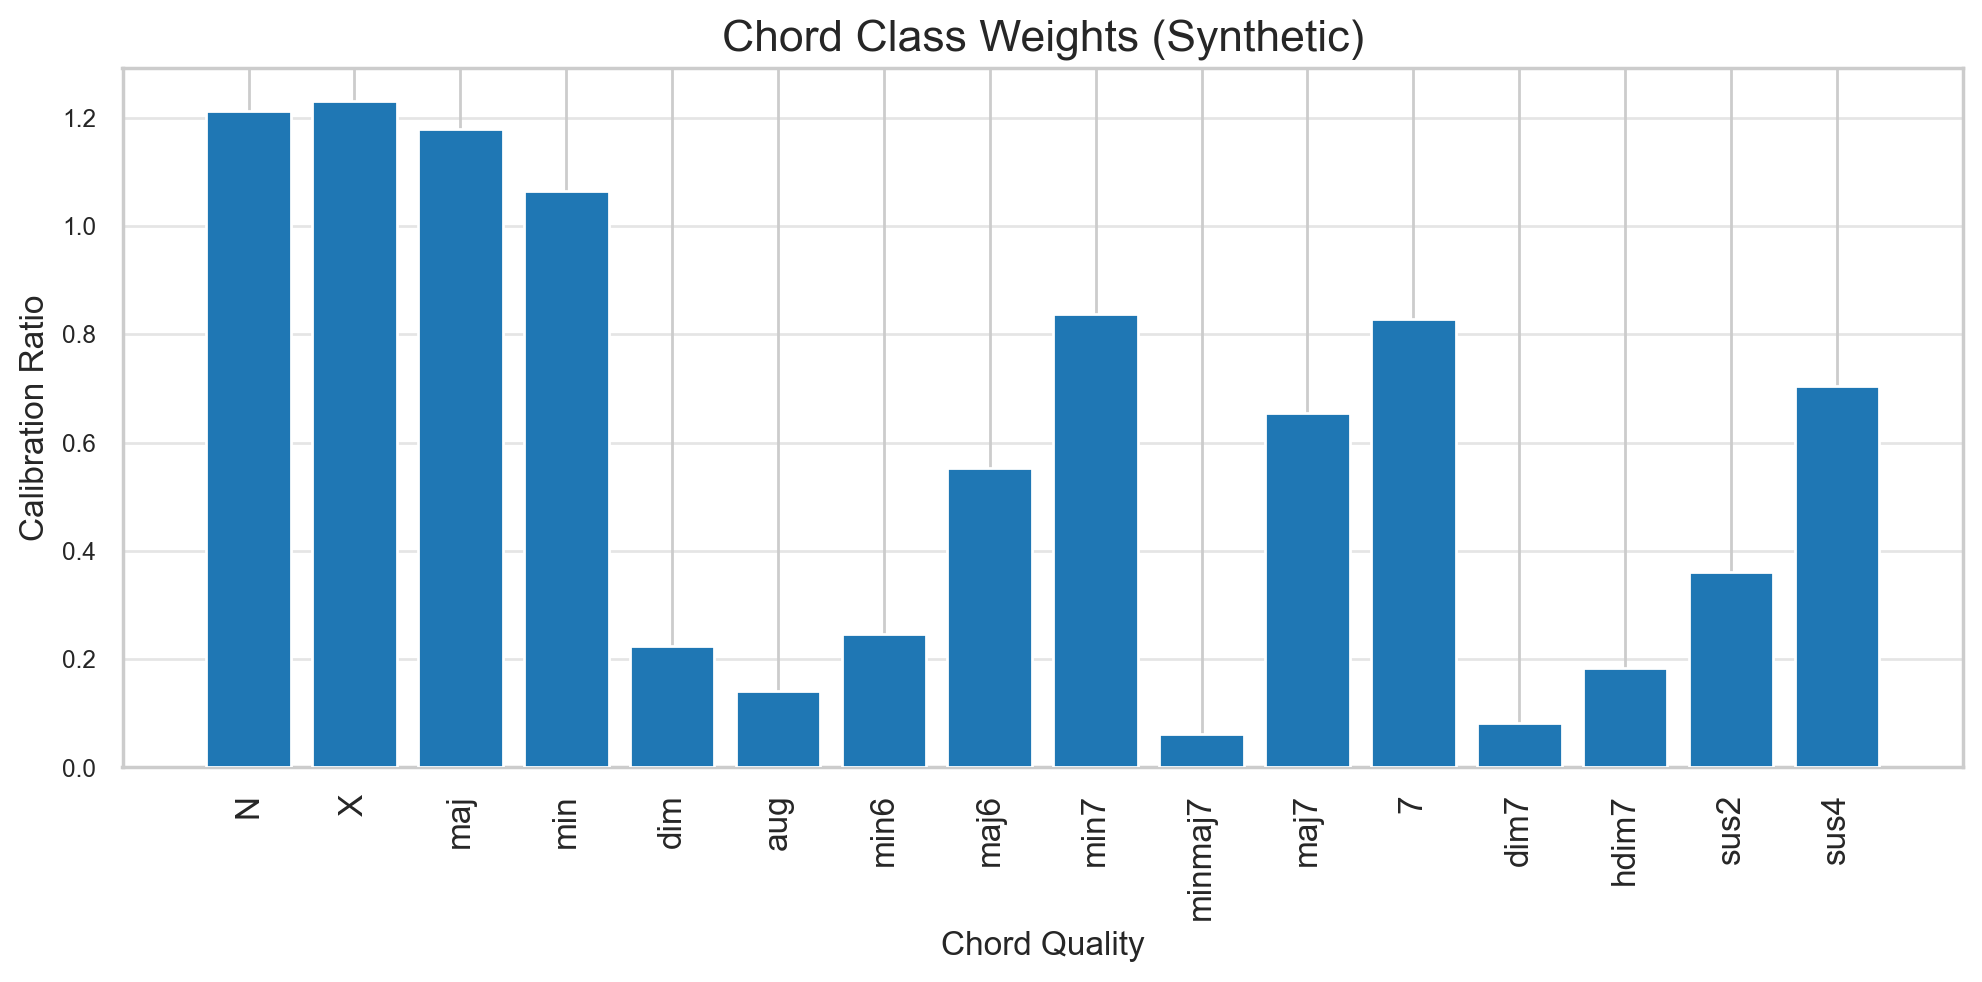
\includegraphics[width=0.8\textwidth]{figures/calibration_ratios.png}
    \caption{Calibration ratios $r_q$ of the model's outputs to account for distribution shift. The high ratio on rare chord qualities like \texttt{majmin} show that these qualities are much more common in the synthetic dta.}\label{fig:calibration}
\end{figure*}

\subsection{Difference in Confusion Matrices with Synthetic Data}\label{app:cm_synthetic_data}

Figure~\ref{fig:cm_synthetic_data} compares the normalised confusion matrices of models trained with and without synthetic data. Incorporating synthetic data reduces predictions of \texttt{X} chords and improves recall for \texttt{min7} and \texttt{dim} qualities, but degrades performance on \texttt{hdim7} and \texttt{min6}. It also shifts certain errors, notably from \texttt{min} to \texttt{maj} in \texttt{7} and \texttt{min7} cases. Despite these changes, overall accuracy remains unchanged, making it unclear which model performs better overall.

\begin{figure*}[h]
    \centering
    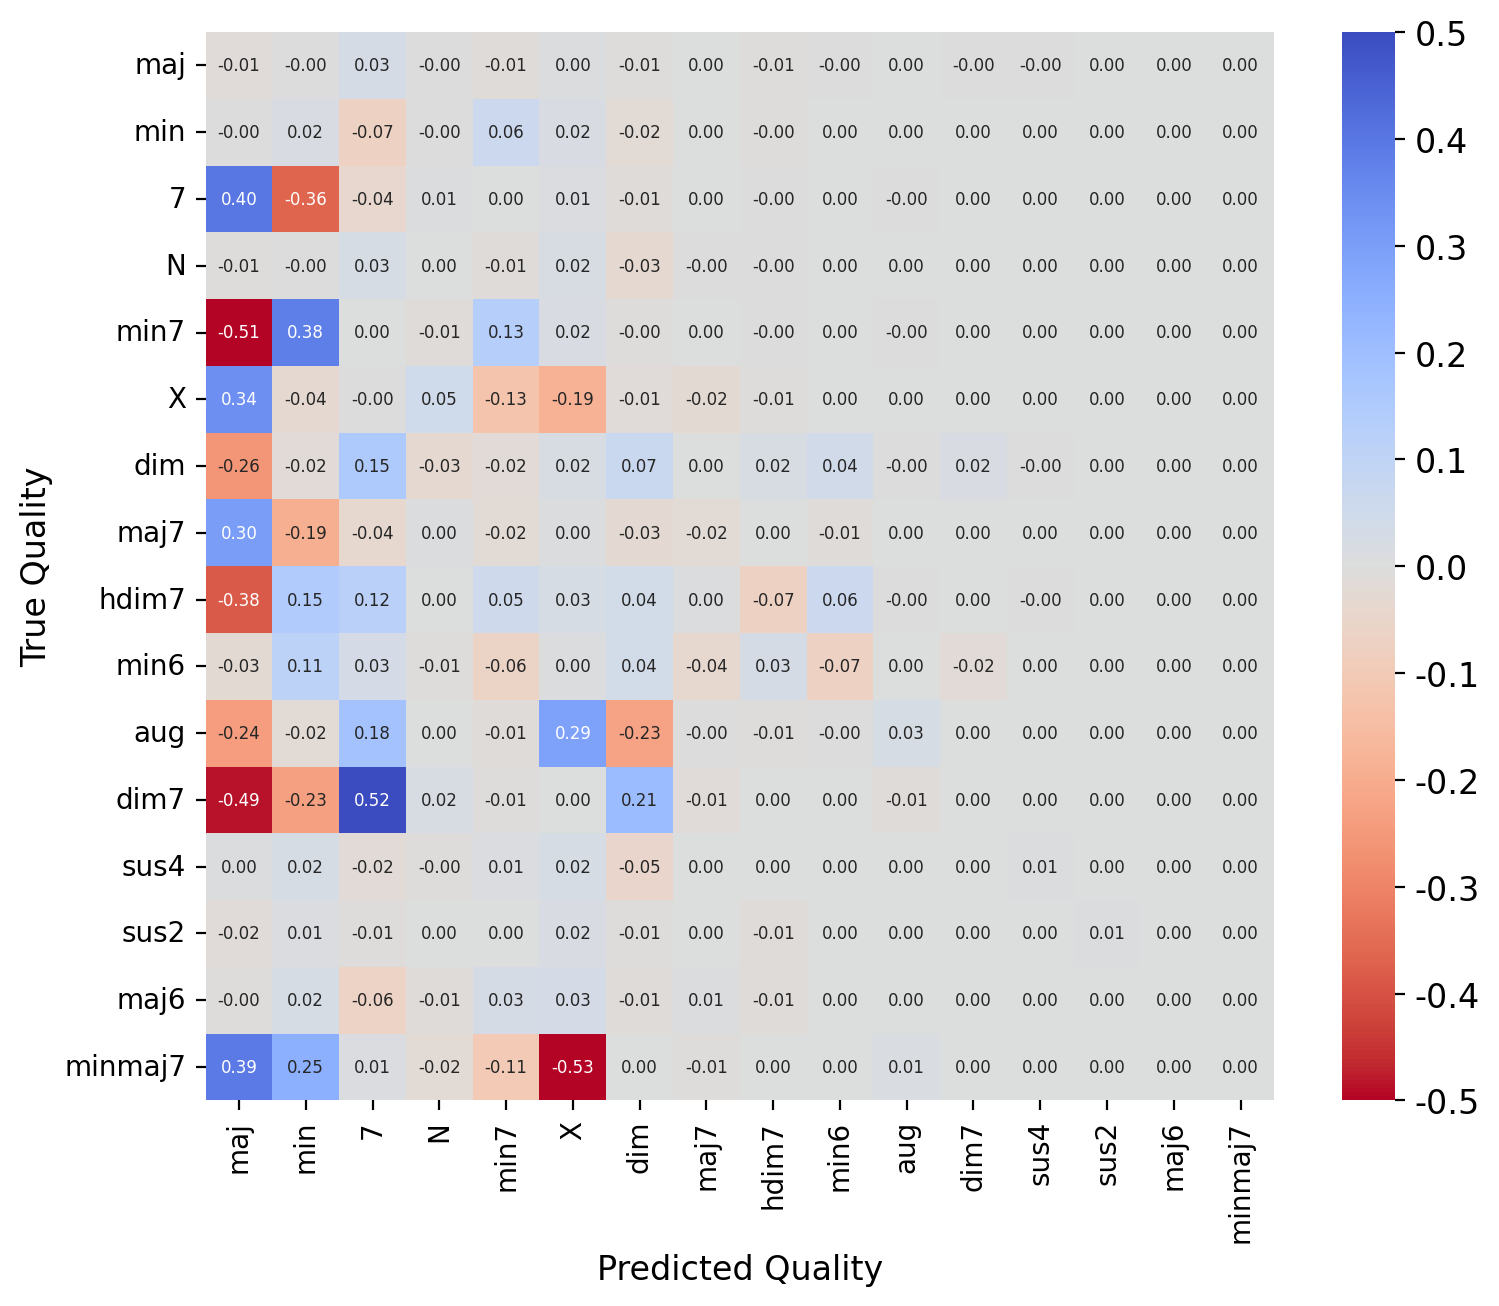
\includegraphics[width=0.8\textwidth]{figures/confusion_matrix_synth.png}
    \caption{Element-wise difference in normalised confusion matrix of the model trained on synthetic data and \emph{pop} data versus just \emph{pop} data with a weighted loss function. There are some notable differences. Training on synthetic data strongly discourages the model from predicting \texttt{X} chords, which are not present in the synthetic data. Recall on \texttt{min7} qualities increases by $13\%$ and by $7\%$ on \texttt{dim} qualities. However, recall \texttt{hdim7} and \texttt{min6} worsens. In general, the model predicts \texttt{maj} less often for rarer qualities. Another interesting observation is that the synthetic data corrects many of the predictions on \texttt{7} qualities from erroneous predictions of \texttt{min} to erroneous predictions of \texttt{maj}. Something similar happens with \texttt{min7} qualities. It is hard to say which model is better. Indeed, their overall accuracies are the same.}\label{fig:cm_synthetic_data}
\end{figure*}

\end{document}
